%%
%% This is file `sample-sigplan.tex',
%% generated with the docstrip utility.
%%
%% The original source files were:
%%
%% samples.dtx  (with options: `sigplan')
%% 
%% IMPORTANT NOTICE:
%% 
%% For the copyright see the source file.
%% 
%% Any modified versions of this file must be renamed
%% with new filenames distinct from sample-sigplan.tex.
%% 
%% For distribution of the original source see the terms
%% for copying and modification in the file samples.dtx.
%% 
%% This generated file may be distributed as long as the
%% original source files, as listed above, are part of the
%% same distribution. (The sources need not necessarily be
%% in the same archive or directory.)
%%
%% The first command in your LaTeX source must be the \documentclass command.
\documentclass[sigplan]{acmart}
\settopmatter{printacmref=false, printfolios=false}
%%
%% \BibTeX command to typeset BibTeX logo in the docs
\AtBeginDocument{%
  \providecommand\BibTeX{{%
    \normalfont B\kern-0.5em{\scshape i\kern-0.25em b}\kern-0.8em\TeX}}}

%% Rights management information.  This information is sent to you
%% when you complete the rights form.  These commands have SAMPLE
%% values in them; it is your responsibility as an author to replace
%% the commands and values with those provided to you when you
%% complete the rights form.
\acmYear{2021}\copyrightyear{2021}
\setcopyright{acmlicensed}
\acmConference[PPoPP '21]{26th ACM SIGPLAN Symposium on Principles and Practice of Parallel Programming}{February 27--March 3, 2021}{Virtual Event, Republic of Korea}
\acmBooktitle{26th ACM SIGPLAN Symposium on Principles and Practice of Parallel Programming (PPoPP '21), February 27--March 3, 2021, Virtual Event, Republic of Korea}
\acmPrice{15.00}
\acmDOI{10.1145/3437801.3441620}
\acmISBN{978-1-4503-8294-6/21/02}

%%
%% Submission ID.
%% Use this when submitting an article to a sponsored event. You'll
%% receive a unique submission ID from the organizers
%% of the event, and this ID should be used as the parameter to this command.
%%\acmSubmissionID{123-A56-BU3}

%%
%% The majority of ACM publications use numbered citations and
%% references.  The command \citestyle{authoryear} switches to the
%% "author year" style.
%%
%% If you are preparing content for an event
%% sponsored by ACM SIGGRAPH, you must use the "author year" style of
%% citations and references.
%% Uncommenting
%% the next command will enable that style.
%%\citestyle{acmauthoryear}

%%
%% end of the preamble, start of the body of the document source.

\usepackage{tabularx}
\usepackage{booktabs}
\usepackage{subcaption}
\usepackage{xspace}
\usepackage{mathtools}
\usepackage{algorithm}
\usepackage[noend]{algpseudocode}

\newcommand{\CC}{C\nolinebreak\hspace{-.05em}\raisebox{.4ex}{\tiny\bf +}\nolinebreak\hspace{-.10em}\raisebox{.4ex}{\tiny\bf +}}
\def\CC{{C\nolinebreak[4]\hspace{-.05em}\raisebox{.4ex}{\tiny\bf ++}}}

\newcommand{\gathercoll}{Gather\xspace}
\newcommand{\allgather}{Allgather\xspace}
\newcommand{\scatter}{Scatter\xspace}
\newcommand{\reduce}{Reduce\xspace}
\newcommand{\broadcast}{Broadcast\xspace}
\newcommand{\reducescatter}{Reducescatter\xspace}
\newcommand{\allreduce}{Allreduce\xspace}
\newcommand{\alltoall}{Alltoall\xspace}

\newcommand{\dgxone}{DGX-1\xspace}
\newcommand{\dgxtwo}{DGX-2\xspace}
\newcommand{\amd}{AMD\xspace}

\newcommand{\chunkstep}[2]{$#1$-chunk $#2$-step\xspace}


\newcommand{\tool}{SCCL}
\newcommand{\toollong}{Synthesized Collective Communication Library}

\newcommand{\setwhere}{\;|\;} % the bar in middle of set builder notation
\newcommand{\qst}{\;} % the "such that" symbol for quantifiers. Could also be . or :
\newcommand{\powerset}{\mathcal{P}}
\newcommand{\posint}{\mathbb{Z}_{\geq0}}
\newcommand{\oftype}{\mathbin{:}}
\newcommand{\range}[1]{\left[#1\right]}
\newcommand{\dotscend}{\dotsc\hspace{-0.08em}}

\newcommand{\Ite}[3]{\mathrm{ITE}(#1,#2,#3)}
% \newcommand{\Ite}[3]{\text{if }#1\text{ then }#2\text{ else }#3}

% Synthesis stuff
\newcommand{\collectiveproblem}{\textsc{SynColl}\xspace}
\newcommand{\bcastproblem}{\textsc{SynCollBcast}\xspace}
\newcommand{\reducingproblem}{\textsc{SynCollReduce}\xspace}
\newcommand{\size}{P}
\newcommand{\ids}{I}
\newcommand{\pre}{\mathit{pre}}
\newcommand{\post}{\mathit{post}}
\newcommand{\chunk}{C}
\newcommand{\gchunk}{G}
\newcommand{\toglobal}{\mathit{ToGlobal}}
\newcommand{\steps}{S}
\newcommand{\rounds}{R}
\newcommand{\fb}{k}
\newcommand{\bw}{B}
\newcommand{\rparts}{Q}
\newcommand{\sends}{T}
\newcommand{\start}[2]{\mathit{time}_{#1,#2}}
\newcommand{\send}[3]{\mathit{snd}_{#1,#2,#3}}
\newcommand{\qouta}{\mathit{Q}}

\newcommand{\broadcasting}{non-com\-bin\-ing\xspace}
\newcommand{\broadcastingCap}{Non-com\-bin\-ing\xspace}
\newcommand{\reducing}{com\-bin\-ing\xspace}
\newcommand{\reducingCap}{Com\-bin\-ing\xspace}

\newcommand{\etal}{\textit{et al}.}


\begin{document}

%%
%% The "title" command has an optional parameter,
%% allowing the author to define a "short title" to be used in page headers.
\title{Synthesizing Optimal Collective Algorithms}

%%
%% The "author" command and its associated commands are used to define
%% the authors and their affiliations.
%% Of note is the shared affiliation of the first two authors, and the
%% "authornote" and "authornotemark" commands
%% used to denote shared contribution to the research.

\author{Zixian Cai}
\authornote{Both authors contributed equally to the paper. 
The work was done during internships at Microsoft Research.} %% \authornote is optional;

%\orcid{0000-0003-2262-2380}             %% \orcid is optional
\affiliation{
  \department{Research School of Computer Science}       %% \department is recommended
  \institution{Australian National University}           %% \institution is required
  \city{Canberra}
  \state{ACT}
  \country{Australia}                   %% \country is recommended
}
\email{zixian.cai@anu.edu.au}          %% \email is recommended

%% Author with single affiliation.
\author{Zhengyang Liu}
\authornotemark[1]
\affiliation{
  \department{School of Computing}              %% \department is recommended
  \institution{University of Utah}            %% \institution is required
  \city{Salt Lake City}
  \state{UT}
  \country{USA}                    %% \country is recommended
}
\email{liuz@cs.utah.edu}          %% \email is recommended



\author{Saeed Maleki}

\affiliation{
  \institution{Microsoft Research}           %% \institution is required
  \city{Redmond}
  \state{WA}
  \country{USA}                   %% \country is recommended
}
\email{saemal@microsoft.com}         %% \email is recommended

\author{Madanlal Musuvathi}

\affiliation{
  \institution{Microsoft Research}           %% \institution is required
  \city{Redmond}
  \state{WA}
  \country{USA}                   %% \country is recommended
}
\email{madanm@microsoft.com}         %% \email is recommended

\author{Todd Mytkowicz}
\affiliation{
  \institution{Microsoft Research}           %% \institution is required
  \city{Redmond}
  \state{WA}
  \country{USA}                   %% \country is recommended
}
\email{toddm@microsoft.com}         %% \email is recommended

\author{Jacob Nelson}
\affiliation{
  \institution{Microsoft Research}           %% \institution is required
  \city{Redmond}
  \state{WA}
  \country{USA}                   %% \country is recommended
}
\email{jacob.nelson@microsoft.com}         %% \email is recommended

\author{Olli Saarikivi}

\affiliation{
  \institution{Microsoft Research}           %% \institution is required
  \city{Redmond}
  \state{WA}
  \country{USA}                   %% \country is recommended
}

\email{olsaarik@microsoft.com}         %% \email is recommended
%

%%
%% By default, the full list of authors will be used in the page
%% headers. Often, this list is too long, and will overlap
%% other information printed in the page headers. This command allows
%% the author to define a more concise list
%% of authors' names for this purpose.
\renewcommand{\shortauthors}{Zixian Cai, Zhengyang Liu \etal}

%%
%% The abstract is a short summary of the work to be presented in the
%% article.
\begin{abstract}
Modern computer architectures are complex, with a wide range of
features that can be leveraged to optimize software performance.
However, efficiently optimizing software for these architectures
remains a challenging task. Traditional optimization techniques,
such as manual optimization by human experts or optimization by
compilers, may not fully exploit the unique features of novel
architectures, leading to suboptimal performance.

Program synthesis is a promising approach to address this challenge.
At its core, program synthesis searches for programs that meet a
specified set of requirements. Recent advances in SMT solvers and
increased computation power have made program synthesis a viable
choice for code generation. Program synthesis can generate code
specifically tailored to the target architecture, leveraging
domain-specific knowledge and advanced search techniques to create
highly optimized code.

The overall goal of this dissertation is to develop program
synthesizers that efficiently optimize software for emerging
architectures. The thesis statement of my dissertation is that program
synthesis can be used to generate highly optimized code for novel
architectures, outperforming traditional optimization techniques. To
achieve this goal, I develop program synthesizers that can
generate optimized code for a variety of hardware platforms. I
evaluate the effectiveness of these synthesizers by comparing the
generated code with manually optimized code and code generated by
traditional compilers. The results show that program synthesis can
produce code that is faster and more efficient than code generated by
traditional optimization techniques.

I present Minotaur, a superoptimizer that uses program synthesis
to optimize LLVM IR code. Minotaur extracts program slices from LLVM IR
code, and uses an SMT solver to find optimized versions of these slices.
Minotaur is designed to work within the LLVM optimization pipeline, and
can be used to discover new optimizations that are missed by traditional
compilers.

We present SCCL, a program synthesizer that optimizes collective
algorithms for parallel computation. SCCL uses domain-specific knowledge
about collective algorithms to generate highly optimized code for
specific architectures. SCCL is designed to be a drop-in replacement for
existing collective communication libraries, such as NVIDIA NCCL and AMD RCCL,
and can be used to improve the communication performance of parallel
applications.

\end{abstract}

%%
%% The code below is generated by the tool at http://dl.acm.org/ccs.cfm.
%% Please copy and paste the code instead of the example below.
%%

\begin{CCSXML}
<ccs2012>
<concept>
<concept_id>10010520.10010521.10010528.10010530</concept_id>
<concept_desc>Computer systems organization~Interconnection architectures</concept_desc>
<concept_significance>500</concept_significance>
</concept>
<concept>
<concept_id>10011007.10010940.10010971.10010972.10010973</concept_id>
<concept_desc>Software and its engineering~Cooperating communicating processes</concept_desc>
<concept_significance>500</concept_significance>
</concept>
</ccs2012>
\end{CCSXML}

\ccsdesc[500]{Computer systems organization~Interconnection architectures}
\ccsdesc[500]{Software and its engineering~Cooperating communicating processes}

%%
%% Keywords. The author(s) should pick words that accurately describe
%% the work being presented. Separate the keywords with commas.
\keywords{GPU, Synthesis, Collective Communication, Interconnection, Network}

%% A "teaser" image appears between the author and affiliation
%% information and the body of the document, and typically spans the
%% page.

%%
%% This command processes the author and affiliation and title
%% information and builds the first part of the formatted document.
\maketitle

\section{Introduction}
% Machine learning workloads imply novel topologies
Recent trends in machine learning towards training and serving large models together with the stagnation of Moore's-law-induced compute performance has led system designers to include novel high-bandwidth interconnect networks both within and across nodes in distributed clusters. For instance, a \dgxone server consists of two x86 processors and eight GPUs, interconnected by NVIDIA's NVLink network as shown in Figure~\ref{fig:dgx1-topo}. These networks' designs are motivated as much by the need to perform efficient \allreduce, a crucial primitive in machine learning, as well as by hardware considerations such as signal integrity, cooling and physical layout.
%\todo{only NVLink is shown in the figure, maybe reword the sentence or change the figure?
%Actually, I am not even sure if a socket contains THOSE four GPUs.}
A wide variety of similar accelerators with novel high-speed interconnects are used to train machine learning models today, including AMD's MI50 GPUs~\cite{mi50}, Graphcore's IPUs~\cite{graphcore} and Google's TPUs~\cite{tpu}.
%\todo{We mention distributed clusters but don't otherwise address them in the paper, I think}

% Hand-written communication primitives - what are the problems.
These novel topologies require novel communication kernels to maximize performance. Today these kernels are written and optimized manually. For instance, NVIDIA Collective Communication Library (NCCL) has two general algorithms for the supported operations such as \allreduce: a high-bandwidth ring algorithm and a low-latency tree algorithm. These implementations are manually written and they do not necessarily have the best performance for different topologies including \dgxone's. On one hand, repeating this manual effort for other communication primitives such as \alltoall or extending already implemented algorithms to a wide variety of hardware topologies is simply infeasible.
%\todo{maybe just say communication algorithms, as ring/tree algorithms are mentioned later}

On the other hand, optimizing these communication kernels for performance for each topology and buffer size is crucial. For instance, we found 30\% of the training time for the 8.3 billion parameter Megatron language model with model parallelism is spent inside \allreduce where each
buffer is of medium size (10-100MB). Also, for data parallelism, the communication buffers
could range from a few KBs (one layer) to a few GBs (the entire model).
We expect this wide range of sizes as large models are developed and trained on
larger distributed clusters.

%As machine learning models growing both in size and training complexity, the
%potential payoffs for such automation are significant in our current world. For
%example, when the 8.3 billion parameter Megatron language model is trained with
%8-way model parallelism on an NVIDIA DGX-1~\cite{megatronlm-arxiv}, 30\% of the
%training time is spent on communication.

%GPUs are used to accelerate a wide variety of tasks, from machine learning to
%simulations for engineering and physics. As the complexity of these tasks grows,
%there is a trend to pack an increasing number of GPUs inside a single node. This
%in turn places increasing importance on the mechanisms for GPU-to-GPU
%communication.

%In contrast with traditional inter-node networks, the interconnects for GPUs
%inside a node are often highly asymmetric. This is caused by a number of
%concerns, such as limitations on wire length and signal quality requirements for
%high-bandwidth links such as PCIe and NVLink as well as limitations on GPU
%placement due to cooling and physical layout. This results in in-node networks
%often not corresponding to any widely studied network topology (e.g., butterfly
%or hypercube). \todo{Give an example here?}

%Just like in traditional networks, the communication patterns have to be
%tailored to the topology for maximum performance. This has been done in isolated
%cases as, for example, NVIDIA Collective Communication Library (NCCL) implements
%algorithms optimized for their 8 GPU DGX-1 servers (see Figure~\ref{fig:dgx1-topo}). However, the wide variety of
%available hardware targets means that it is hard for a library to provide
%optimal algorithms for all configurations, which makes this an ideal target for
%automation.

\begin{figure}[tbp]
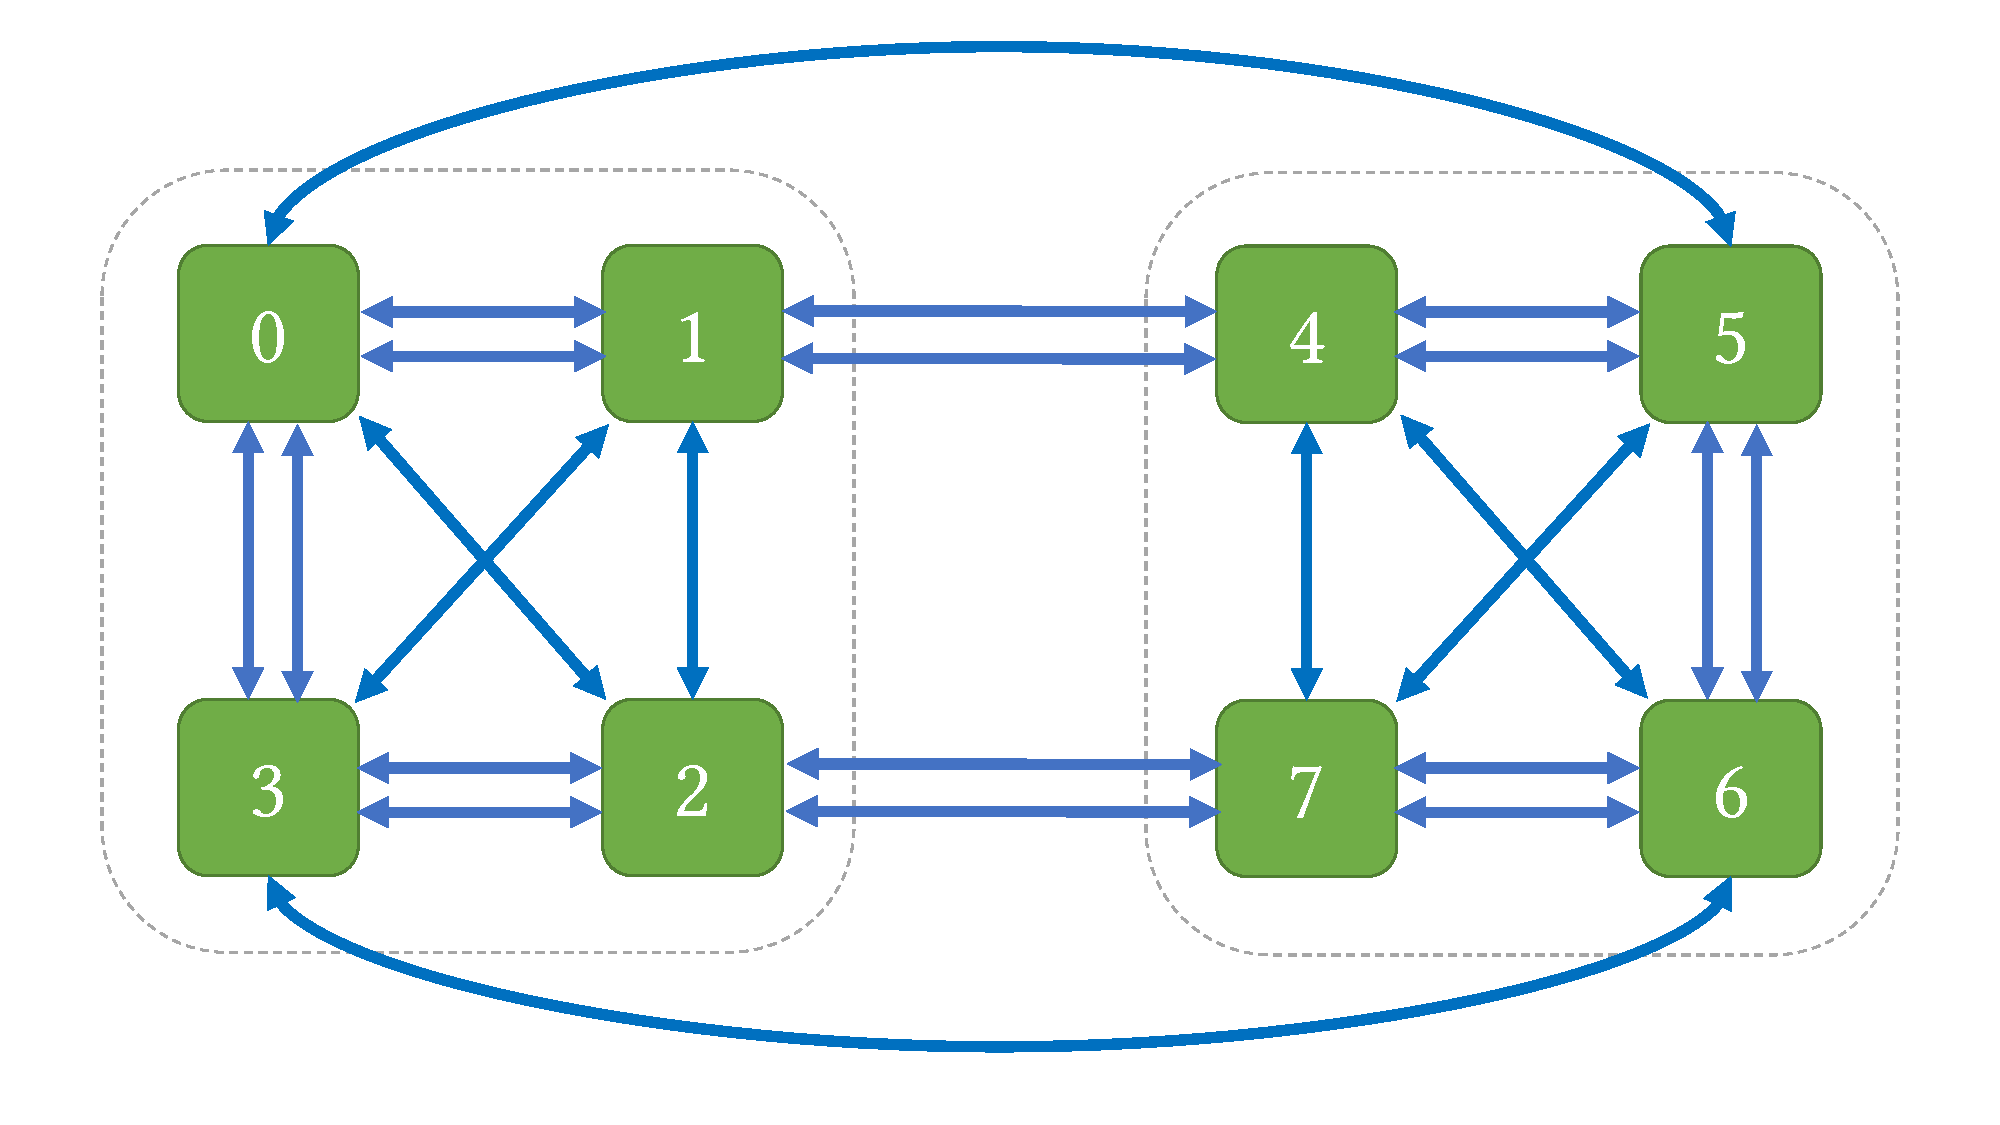
\includegraphics[page=1,width=\columnwidth]{figures/topos.pdf}
\caption{NVLink topology of an NVIDIA DGX-1.}
\label{fig:dgx1-topo}
\end{figure}
%\todo{the grey box indicating a socket has a low contrast when printed. colours for two different rings should have higher contrast (blue and orange perhaps?)}

% explain our approach
In this chapter, we automatically synthesize high-performance communication kernels.
Given a topology, specified as a graph with bandwidth constraints on nodes and edges, and a communication primitive, specified as the pre- and post-condition on data location and computation on it, we generate~(Section~\ref{sec:synthesis}) a quantifier-free SMT formula that captures the set of all feasible algorithms that implement the primitive on the input topology.
Exploring this space to appropriately minimize the number of communication steps or decrease the granularity of communication at each step, is a computationally difficult problem. We exploit
an SMT solver to synthesize algorithms that explore this tradeoff along the Pareto frontier between latency-optimality and bandwidth-optimality.
For every solution from the SMT solver, we automatically generate and lower~(Section~\ref{sec:lowering}) high-performance implementations.


% We approach this problem as a synthesis problem. Collective communication
% primitives can be specified in terms of pre- and post-conditions on which
% processes data resides on and optionally where a user specified reduction
% function has been applied. We encode pre- and post-conditions as well as actions
% to move data between processes as quantifier-free SMT formulas, which we solve
% using Z3. We further impose constraints on bandwidth usage based on the topology
% of the specific machine we are targeting and limit the number of steps for the
% whole algorithm. This gives us a way to explore the entire space of possible
% algorithms for implementing a given primitive on the target hardware.

% how do we make it scalable
When using SMT, finding the right encoding can make all the difference for the
feasibility of an approach. This paper details the important design choices in
our encoding that help it scale to all of our hardware targets. We use the SMT
encoding for \broadcasting collectives, such as \broadcast, while for \reducing
collectives, such as \reduce, we employ a reduction back to the synthesis
problem for \broadcasting collectives.
%A key observation is that topologies have natural symmetries. Our encoding exploits this symmetry to efficiently explore the space of algorithms without sacrificing satisfiability.
This reduction generalizes a well known fact that some \reducing collectives may
be produced by inverting a \broadcasting one, e.g. \reduce by inverting \broadcast.

%This allows us to reuse
%the synthesis of certain primitives such as \allreduce, further improving our
%scalability.
%\todo{"time time-reversed mirror-image", huh? find easier to understand wording.}
%\todo{what do you mean by "modularize"? it's more like we reduce (no pun intended) the problem of reduction to broadcasting, which is the wording used later in bullet points}

% This informed an optimization in
% our encoding, that allows us to make reasoning about which GPUs data has been
% reduced implicit.

%\todo{This is quite vague right now.}

% The ability to control the number of steps an algorithm must execute in gives us
% a novel capability for trading off between latency and bandwidth optimality. By
% synthesizing a range of algorithms at different points in this space we can use
% the best algorithm for any given message size. While MPI implementations and
% NCCL both switch between algorithms based on message size, our synthesis
% approach allows us to do so in a much more fine grained manner. We show that
% this enables our algorithms to provide better performance than NCCL at all
% message sizes. \todo{Update this claim with truth.}

We implement our approach in a tool called \toollong{}~(\tool{}),
which probes the target hardware topology, synthesizes algorithms for
it using Z3~\cite{z3} and finally generates CUDA code that efficiently implements that algorithm.  These algorithms are
synchronous; at every step of the algorithm, one or more of the nodes
send and/or reduce data from others.
%\todo{"CUDA code"=>hardware dependent code? we have AMD GPUs. From saemal: AMD runs CUDA. OpenCL is another possibility but no one really uses it.}

% algorithmic novelty
Some of the algorithms we synthesize are novel, with no known counterparts in
the literature occupying the same latency-bandwidth tradeoff. For example, we
have produced a latency-optimal 2-step (4-step) algorithm for
the \allgather (\allreduce) primitive in the DGX-1 topology (Figure~\ref{fig:dgx1-topo}) and
a bandwidth-optimal 3-step (6-step) algorithm for the \allgather (\allreduce) primitive on the
same topology.  In addition to providing novel
algorithms, our approach informs us when a combination of bandwidth and number
of steps is \emph{not possible}. This makes our synthesis approach a tool for
probing the algorithmic properties that a given topology provides, which is
useful for co-design of hardware interconnects with communication libraries.
%\todo{"occupying the same latency-bandwidth tradeoff": exhibiting? and being different isn't necessarily good, we want more bandwidth with the same latency or lower latency with the same bandwidth.}
%\todo{tell reader that the "number of steps" correlate with latency?}
% results
Our evaluation~(Section~\ref{sec:evaluation}) shows us that this approach scales and beats NCCL in almost all cases.


To summarize, the contributions of this chapter are as follows:
\begin{itemize}
    \item A formalization of the synthesis problem for \broadcasting collectives.
    \item A general strategy for encoding the synthesis problem for
    collective communications algorithms into the quantifier-free linear integer
    arithmetic (QF\_LIA) sub-logic of the SMT-LIB logic.
    \item A reduction from the synthesis problem for \reducing collectives to that for \broadcasting collectives.
    % \item Explanations of some novel algorithms our synthesis has produced.
    \item A description of how \tool{} generates efficient code for the algorithms we synthesize on nodes with NVIDIA or AMD GPUs.
    \item An evaluation of \tool's generated algorithms on common server topologies for deep learning workloads and a comparison against NCCL.
\end{itemize}

%\todo{Paper structure paragraph?}

%%% Local Variables:
%%% mode: latex
%%% TeX-master: "paper"
%%% End:

\section{Overview}
This section provides an overview of synthesizing latency- and bandwidth-optimal algorithms, using \allgather for the
\dgxone topology~(Figure~\ref{fig:dgx1-topo}) as the running example.

\subsection{Collective Communication Primitives}
\label{sec:background-collectives}
Collective communication primitives allow nodes in a networked system to perform operations on shared data. As an example, if each node has some input data, the \allgather primitive transfers these data to all of the nodes.  One way to implement this is for each node to independently send its data to all other nodes. But, an algorithm in which the nodes collectively work together can be more efficient. The efficiency of such algorithms depends on the network topology.

\begin{comment}
    For instance, given a set of nodes each having an array of data, the \allreduce primitive computes the sum (or some specified associative operation) of all these arrays and stores the result in each of these arrays.

Computing the primitives such as \allreduce requires the nodes to communicate. This communication usually happens in smaller chunks of the input array. Given $N$ nodes, say we split the input array into $N$ chunks, where $c_{i,j}$ represents the $i$th chunk at node $j$. One way to compute \allreduce is as follows. First, we compute at node $i$, a partial sum $d_i = \sum_j c_{i,j}$. These reductions can be performed by arranging $N$ nodes in a spanning tree and communicating chunks $c_{i,j}$ along the tree. Note, there are $N$ parallel reductions each possibly using a different spanning tree. This arrangement of reduced data is called the \reducescatter primitive. Once we have the chunks $d_i$, we can perform an \allgather operation by ensuring each node has a copy of $d_i$. In essence, \allgather involves $N$ simultaneous broadcasts of $d_i$ from node $i$. Thus, we have implemented \allreduce by performing an \reducescatter followed by an \allgather.
\todo{I think the ``$N$ parallel reductions each possibly using a different spanning tree'' makes this confusing---is this describing an approach where each node reduces $1/N$ of the chunks?}
\todo{say "compute at node $i$, a partial sum" of chunk $i$.}
\todo{they're are a part of the sum of arrays. they are not really partial sums, in the sense that, e.g., only data from half of the nodes are added.}
\todo{"there are $N$ parallel reductions"=>these $N$ parallel reductions}

Implementing a collective communication primitive depends on the topology. For instance, when executing parallel reductions or broadcasts in the implementation above, the algorithm has to choose different spanning trees to utilize the bandwidth on all links in the topology. Similarly, the algorithm has to choose the ideal chunk size to use for communication. We will demonstrate these choices for the \dgxone topology described below.
\todo{"Implementing" $\ldots$ efficiently}
\todo{"has to chose ": might have to choose}
\end{comment}

\subsection{Topology}
The network topology specifies how the nodes are connected with each other and the latency and bandwidth constraints on the links connecting them. Consider the \dgxone topology shown in Figure~\ref{fig:dgx1-topo}. It consists of $8$ GPUs (or nodes, in the above formalism) split into two groups $\{0,1,2,3\}$ and $\{4,5,6,7\}$. The nodes in each group are fully connected. In addition, there are four inter-group links as shown in the figure. These nodes are connected through
NVLinks, with some nodes connected with two parallel NVLinks as shown in Figure~\ref{fig:dgx1-topo}.

%There are two kinds of links shown in two different colors. The fast links, such as the one connecting nodes $0$ and $1$ have twice the bandwidth as the (relatively) slow links, such as the one connecting nodes $0$ and $2$. The figure represents the fast links with two arrows. Each link is bidirectional allowing concurrent sends and receives at full bandwidth.
%\todo{Remove the colors and the double arrow should make it clear}
%\todo{Also just mention that they are called nv2 and nv1 links}
%\todo{"split into two" groups, each associated with one CPU socket.}
%\todo{"All the nodes within a socket": all the GPUs in the same group}
%\todo{"inter-socket links" sound like QPI: maybe inter-group?}
%\todo{also check the usage in latency-optimal algorithm}
%\todo{I recommend talking about these in terms of groups rather than sockets to avoid the NVLink/PCIe/QPI confusion too -jn}
%\todo{I also recommend not talking about ``fast'' and ``slow'' links, since the diagram shows a fast link as 2 slow links (which is indeed what it is), and we then talk about using 6 logical rings; better to just say 6 links and 6 rings}

The \dgxone's design was heavily influenced by the need to do gradient reduction for machine learning workloads. Specifically, this topology forms two non-overlapping rings: one connecting nodes $\{0,1,4,5,6,7,2,3\}$ with two NVLinks per edge and another connecting $\{0,2,1,3,6,4,7,5\}$ with one NVLink per edge. These rings are bidirectional and thus form $6$ logical single-NVLink rings. The NCCL library implements \allgather by running $6$ simultaneous ring algorithms as we discuss below.

%Given the fast ring has twice the bandwidth and each ring is bidirectional, this allows the implementation to utilize $6$ logical rings with the same bandwidth %to implement collection primitives
%(2 from the slow ring and 4 from the fast ring).

\subsection{Cost Model}
%\todo{I think we need to define bandwidth and latency optimality here. My understanding is that a bandwidth-optimal algorithm is one that sends the minimal amount of data necessary to complete its operation, and a latency-optimal one uses the fewest number of communication rounds possible to complete its operation. Is that what we mean?}

%Before discussing how to build bandwidth- and latency-optimal algorithms for this topology, we will introduce a simple cost model.
We will characterize the communication cost using the $(\alpha, \beta)$ model~\cite{hockney1994communication}. That is, sending a message of size $L$ along a link costs $\alpha + L\cdot\beta$ time.
Here, $\alpha$ is the latency of communication and captures the {\em fixed} costs, such as the overhead of initiating a transfer or invoking a GPU kernel,
and $\beta$ is the inverse bandwidth of the link and captures {\em per-byte} costs, such as copying data into system buffers. Li \etal{} extensively studies the transfer time of buffers with
different sizes over numerous GPU interconnections\cite{alphabeta}. Their result show that with NVLinks, the transfer time stays almost constant up-to a large buffer size and only then it start to increase linearly.
These results confirm that the $(\alpha,\beta)$ model is suitable for characterizing communication cost over NVLinks.

The cost of a collective algorithm for an input of size $L$ will be of the form $a\cdot\alpha + b \cdot L \cdot \beta$. We call $a$ the {\em latency cost} of the algorithm and $b$ the {\em bandwidth cost} of the algorithm. Given a class of algorithms that implement a collective on a given topology, an algorithm is {\em latency-optimal} ({\em bandwidth-optimal}) if no other algorithm in the class has a lower latency (bandwidth) cost. Usually, there is a tradeoff between the latency cost and the bandwidth cost when designing collective algorithms.  An algorithm with latency cost $a$ and bandwidth cost $b$ is said to be {\em Pareto-optimal} with respect to a class of algorithms if for every algorithm in the class with latency cost $a'$ and bandwidth cost $b'$, we have $a = a' \Rightarrow b' \geq b$ and $b = b' \Rightarrow  a' \geq a$.

%The $\alpha$ term represents the {\em fixed} cost of sending a message from the overhead of invoking a GPU kernel to the latency across the network. The $beta$ term represents from the cost of copying data across system buffers to the time taken to transmit the bytes at a given network bandwidth. For small message sizes, the cost is determined by the fixed cost $\alpha$, while for large message sizes, the cost is determined by the per-byte cost $\beta$.
%\todo{we are going to have a single kernel launch, so many not the kernel launch cost?}
%\todo{give our estimation of $\alpha$ and $\beta$ cost for DGX1 and NVLinks.}
%\todo{the from $\ldots$ to $\ldots$ in a long sentence is confusing: consider "such as"}
%\todo{note: I replaced ``packet'' with ``message'', since alpha is more about the cost to initiate a transfer rather than to send a single 256-byte NVLink packet}

\subsection{Bandwidth-Optimal Algorithm for \dgxone}
\label{sec:motivation:bw-optimal}
As described above, the \dgxone topology has $6$ logical rings. \allgather for one ring can be implemented as follows. Each node simultaneously sends its data to the next node in the ring. In subsequent steps, each node stores the received data and sends it to the next node in the ring. In $7$ steps all nodes will have received data from all of the other $7$ GPUs. The $6$-ring algorithm is a generalization of this algorithm. Each node splits its data into $6$ chunks and executes the ring algorithm along each of the $6$ rings, with one chunk per ring. If $L$ is the size of the input data, each ring algorithm takes $7$ steps and communicates $\frac{L}{6}$ bytes. Thus, the cost of the $6$-ring algorithm is
$$7\cdot \alpha + \frac{7}{6}\cdot L \cdot \beta$$

Each node has to receive at least $7 \cdot L$ amount of data, and it has an agglomerated incoming per-byte cost of $\beta/6$ (6 incoming NVLinks). Thus, any algorithm for \allgather has to take at least $\frac{7}{6}\cdot L \cdot \beta$ amount of time. Thus, this algorithm is bandwidth-optimal for the \dgxone topology. But can we do better with the latency cost?

Using the techniques described in this paper, we have automatically synthesized an algorithm~(Section~\ref{fig:dgxone:syn}) with cost $$3\cdot \alpha + \frac{7}{6}\cdot L \cdot \beta$$ To the best of our knowledge, this algorithm was not previously known. Moreover, we prove that this algorithm is Pareto-optimal with respect to the class of algorithms we call $k$-synchronous algorithms~(Section~\ref{sec:ksync}).

\subsection{Latency-Optimal Algorithm for \dgxone}
The next question is whether we can improve upon the latency cost of the synthesized algorithm. If each node communicates its data along a binary tree instead of a ring, it would take at least $3$ steps. Using the techniques described in this paper, we have automatically synthesized a better algorithm~(Section~\ref{fig:dgxone:syn}) with cost $$2\cdot \alpha + \frac{3}{2}\cdot L \cdot \beta$$
Since the \dgxone topology has a diameter of $2$, this algorithm is latency-optimal. To the best of our knowledge, a latency-optimal algorithm for the \dgxone was not previously known. This algorithm is Pareto-optimal with respect to the class of $k$-synchronous algorithms.

\begin{comment}
While bandwidth optimal algorithms are suitable for large inputs $D \gg \alpha / \beta$, they are wasteful for small inputs. In such cases, we seek a latency-optimal algorithm. NCCL is
capable of creating trees but on a \dgxone, the created trees are always a line graph and
therefore, they have the same latency as a ring.
\todofor{Saeed}{Does NCCL have a tree based allgather? If not, what's the tree like in allreduce? Is it binary? from saemal: no it does not. For allgather it doesn't even have
any other implementation other than a ring and for allreduce on DGX1, it only creates a ring with the tree. It is safe to say that on DGX-1 they use a ring always even though they have the capability of doing a tree}
\todo{"they are wasteful for small inputs"=>they might not give the smallest possible latency for small inputs}

The technique discussed in this paper synthesized a better algorithm that takes $2$ steps! To the best of our knowledge, this algorithm is not previously known. The algorithm works as follows. In the first step, each node sends its chunk to all its neighbors. For instance, node $0$ sends its chunk to its intra-socket neighbors $1$, $2$, and $3$ as well to its inter-socket neighbor $5$. Since each link is bidirectional communication from nodes do not conflict. At the end of step 1, each node has received chunks from all its intra-socket neighbors and one chunk from its inter-socket neighbor. In the second step, each node sends the chunk from its inter-socket neighbor to all its intra-socket neighbors. That is, node $0$ sends the chunk from $5$ to nodes $1$, $2$, $3$.

This two-step algorithm does not subdivide its input data of size $D$. So, we will call this algorithm a \chunkstep{1}{2} algorithm. The time taken by this algorithm is
$$2\cdot \alpha + 2\cdot D\cdot\beta$$
Since the diameter of this topology is $2$ and each node has to communicate with every other node, one cannot implement an \allgather in one step. Thus, for $D \ll \alpha / \beta$, this algorithm is optimal. We call such algorithms latency optimal.

A natural question, again, is whether a faster latency optimal algorithms exist that can use the bandwidth more efficiently. For instance, the \chunkstep{1}{2} does not make use of fast bandwidth links as it only sends one chunk between a pair of nodes at each step. This paper shows that such an algorithm exist.
\todo{Not true, with rounds, we have a better algorithm.}

\subsection{Pareto Frontier}
\label{sec:pareto}

While the bandwidth-optimal algorithm is suitable for large input sizes and the latency-optimal algorithm is for small input sizes, many interesting inputs might be of sizes in between the two limits. How do design optimal algorithms in such cases? Let us assume that a \chunkstep{c}{s} algorithm implementing a collective on a given topology exists. Using a similar reasoning as above, this algorithm will take time
$$ s\cdot \alpha + \frac{s\cdot D \cdot \beta}{c}$$
Intuitively, we need to reduce $s$ to improve the latency of the algorithm and increase $c$ to improve the bandwidth utilization of the algorithm, while the constraints of the topology and the implemented collective will restrict the feasible pairs $(c,s)$. For instance, as argued above, $s \geq 2$ and $\frac{s}{c} \geq \frac{7}{6}$ when implementing \allgather on the \dgxone topology. In other words, for a given $s$, $c \leq \left\lfloor\frac{6 \cdot s}{7} \right\rfloor$.
\todo{maybe need to justify why all algorithms can be expressed as \chunkstep{c}{s} performance-wise. Suppose different ranks have different number of steps, which takes different durations. Even though you can find the smallest time slice and the corresponding greatest common divisor logical chunk size, the steps now are "logical" steps, and you don't always pay the $\alpha$ cost.}
\todo{our algorithms are BSP. With the concept of rounds, each step might take different amount
of time. Since 1 bw and 2 bw have 2 as their lcm, having equal chunks makes sense. Maybe we should have this in Section 2?}


By trading latency by increasing $s$, one can search for the largest $c$ for which a feasible \chunkstep{c}{s} exists. Each such algorithm maximizes the bandwidth utilization for a given latency. We can increase $s$ till we reach a bandwidth-optimal algorithm. Together, these form a {\em Pareto frontier} of feasible algorithms. Which of these algorithms to use will depend on the size of the input data $D$, the latency $\alpha$ of the network, and the bandwidth $\beta$ of the network.

\subsection{Summary of the Paper}
In this paper, we propose a systematic method to synthesize algorithms in the Pareto-frontier spanning form the latency-optimal algorithm to the bandwidth-optimal algorithm for a given collective on an input topology. We characterize a class of algorithms that captures a broad set of known algorithms and prove Pareto-optimality of both known algorithms and synthesized new algorithms. We automatically generate an implementation of these algorithms that is competitive with manually hand-tuned communication kernels in use today.

\end{comment}


%\subsection{Synthesizing Optimal Algorithms}
%\todofor{Olli}{Summarize our approach to synthesizing algorithms on the pareto frontier.}
%Given a topology, we automatically optimal algorithms in the pareto frontier.  Essentially a summary of the paper.

\section{Algorithm Synthesis}
\label{sec:synthesis}
This section demonstrates a method to synthesize Pareto-optimal
algorithms that implement a collective primitive on a given topology.
The Pareto-optimality is defined with respect to a class of algorithms
we call {\em $k$-synchronous} algorithms.

We distinguish between {\em \reducing} collectives such as \allreduce
and \reducescatter that combine chunks through computation, and {\em
\broadcasting} collectives such as \allgather and \broadcast that
simply transfer data among nodes. We will focus on synthesizing
\broadcasting collectives and show how to derive \reducing collectives
from related \broadcasting ones.

\subsection{$k$-synchronous Algorithms}
\label{sec:ksync}
%automation.
\begin{figure}
    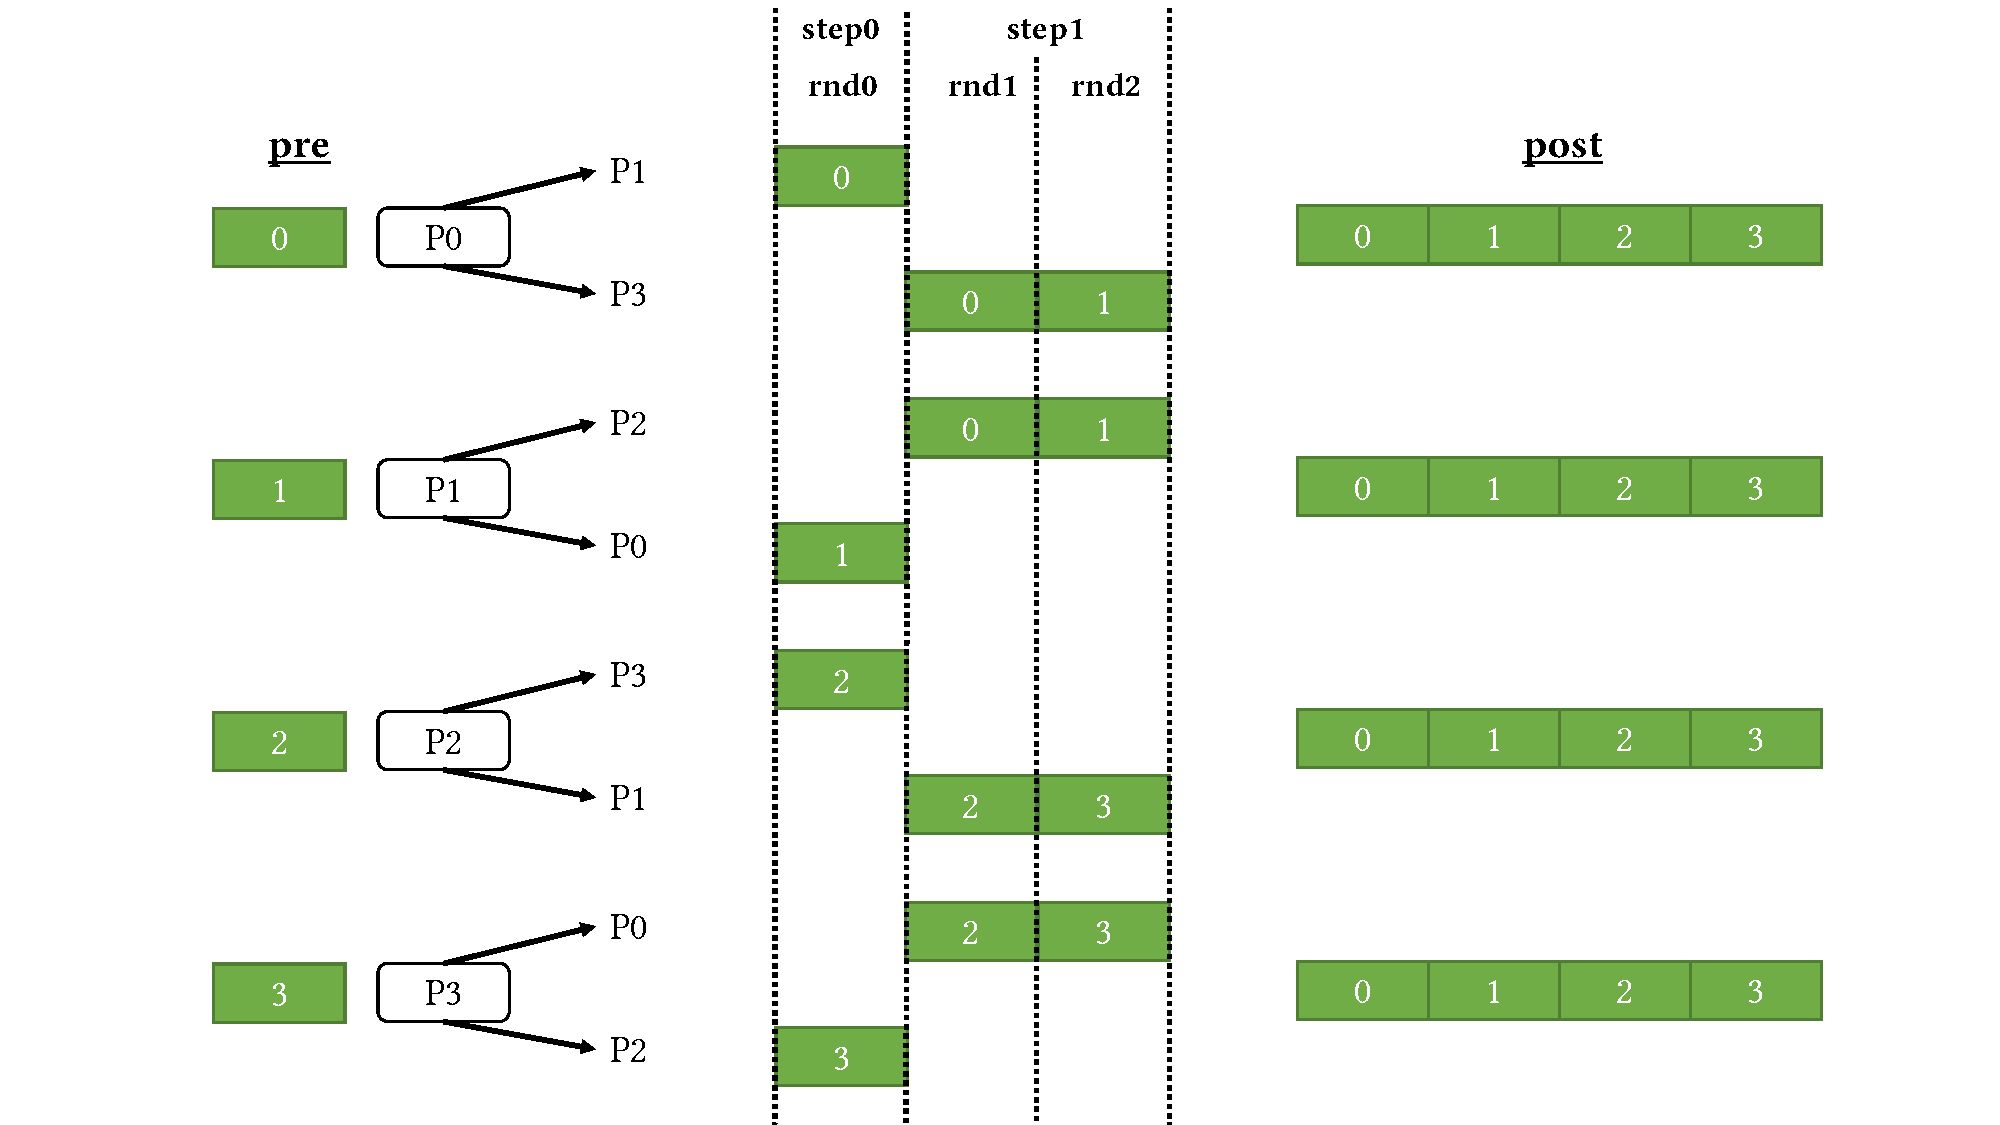
\includegraphics[width=\columnwidth]{figures/allgatherex.pdf}
    \caption{A $1$-synchronous algorithm for \allgather on a ring topology.}
    \label{fig:allgatherex}
\end{figure}

Figure~\ref{fig:allgatherex} shows the
recursive-doubling~\cite{thakur2005optimization} algorithm for
\allgather for a ring topology of four nodes $P0, P1, P2, P3$ with
four bidirectional links of equal bandwidth. This algorithm proceeds
in two {\em steps}. In the first step, nodes at "distance" 1, namely
$P0, P1$ and $P2, P3$ send their data to each other. Each node now has
data from two nodes, which it communicates entirely with nodes at
distance 2, i.e., nodes $P0, P3$ and $P1, P2$ in the second step. At
the end, each node has data from every other node. Since the second
step involves sending twice the amount of data as the first step, we
say it has two \emph{rounds} where in each round, it sends data. Thus,
this step has a total of $3$ rounds. Of the eight (unidirectional)
links, this algorithm uses only four of them per step. To improve
bandwidth utilization, a better option is to split the input data into
equal-sized {\em chunks} and communicate them independently. For
instance, the ring algorithm described in
Section~\ref{sec:motivation:bw-optimal} uses $3$ chunks per node.

The algorithm in Figure~\ref{fig:allgatherex} and many classical
collective algorithms~\cite{thakur2005optimization,chan2007collective}
are instances of {\em synchronous} algorithms. A synchronous algorithm
proceeds in a sequence of synchronous communication {\em steps} with
nodes waiting for other nodes to finish their rounds before starting
the next step. Even if an implementation might not enforce a global
barrier across the nodes, these algorithms choose the amount of data
to communicate per step based on the bandwidth constraints so that the
nodes finish each step at (roughly) the same time.

Many algorithms, like the one in Figure~\ref{fig:allgatherex},
communicate different numbers of chunks per step. We consider each
step as consisting of multiple rounds with each node sending at most
one chunk per unit-bandwidth on its outgoing links. Intuitively, the
number of rounds in an algorithm controls its bandwidth cost, while
the number of steps controls its latency cost. A synchronous algorithm
with $\steps$ steps and $\rounds$ rounds is {\em $k$-synchronous} if
$\rounds \leq \steps + k$. The parameter $k$ limits the amount of
communication per step and allows an SMT solver to effectively search
the space of algorithms bounded by that $k$.
%\todo{Madan mentioned in the chat that for a given $k$, we use it to
%bound $R$. We can make it clearer. The first time I read this, I
%thought we are changing $k$ for some $R$ and $S$ such that $k$ is the
%smallest number such that $R\le S+k$.}

%The terminology of steps and rounds might be confusing at first. The
%best way to distinguish them is to note that in the $(\alpha, \beta)$
%cost model, the latency cost of a $k$-synchronous algorithm depends
%on the number of steps, while the bandwidth cost depends on the
%number of rounds and the number of the chunks.

\subsection{\broadcastingCap Collective Instance}
Now we will provide a uniform formulation for representing
$k$-synchronous algorithms for \broadcasting collectives. An instance
of \collectiveproblem is a tuple
$(\gchunk,\steps,\rounds,\size,\bw,\pre,\post)$, where
\begin{itemize}
    \item[] \hspace{-0.5cm}Parameters:
    \begin{itemize}
    \item $\gchunk\in\posint$ is the global number of chunks
    \item $\steps\in\posint$ is the total number of steps
    \item $\rounds\in\posint$ is the total number of rounds
    \end{itemize}
    \item[] \hspace{-0.5cm}Topology:
    \begin{itemize}
    \item $\size\in\posint$ is the number of nodes
    \item
    $\bw\subseteq\powerset(\range{\size}\times\range{\size})\times\mathbb{N}$
    is the bandwidth relation
    \end{itemize}
    \item[] \hspace{-0.5cm} Specification:
    \begin{itemize}
        \item $\pre\subseteq\range{\gchunk}\times\range{\size}$ is the
        pre-condition
        \item $\post\subseteq\range{\gchunk}\times\range{\size}$ is
        the post-condition
    \end{itemize}
\end{itemize}
Note that for a set $M$ we write $\powerset(M)$ for the power set of
$M$, i.e., the set of all subsets. For an integer $x$, we write
$\range{x}$ for the set $\{0, 1, \ldots, x\}$. Here, $\gchunk, \steps,
\rounds$ are parameters to the desired $k$-synchronous algorithm. The
rest are explained below.

\subsubsection{Topology}
\label{sec:topology}
$\size$ is the number of nodes in the topology. $\bw$ gives a flexible
way to express different bandwidth constraints we have seen in
practice. In its most general form, $\bw$ bounds the sum of chunks
sent along a set of edges in a single round. A point-to-point
communication link from $s$ to $d$ with maximum bandwidth (in chunks
per round) $b$ can be modeled by $(\{(s, d)\}, b) \in \bw$. Some
topologies might limit the net outgoing bandwidth $b$ from a certain
node $s$. If $E$ is the set of outgoing neighbors of $s$, we can model
this by $(\{(s, e) \mid e \in E\}, b) \in \bw$. To model shared bus
topologies, where only one node can send in a round, we include
$(\{(a, b) \mid a \in N, b \in N\}, b)$ in $\bw$ for the set of nodes
$N$ sharing the same link. Note that these constraints are per round,
and when performing $r_i$ rounds in step $i$, we simply multiply the
bandwidth constraint by $r_i$.

\newcommand{\relAll}{All\xspace}
\newcommand{\relRoot}{Root\xspace}
\newcommand{\relScattered}{Scattered\xspace}
\newcommand{\relTranspose}{Transpose\xspace}
\newcommand{\chunkReduce}{\left\lfloor\frac{i}{\size}\right\rfloor}
\begin{table}
    \center
    \begin{tabularx}{\columnwidth}{@{}Xl@{}}
        \toprule
        Name & Relation \\
        \midrule
        \relAll & $\range{\gchunk}\times\range{\size}$ \\
        \relRoot & $\range{\gchunk}\times\{n_\mathit{root}\}$ \\
        \relScattered & $\{(c,n)\in\range{\gchunk}\times\range{\size}
        \setwhere n=c\bmod \size\}$ \\
        \relTranspose & $\{(c,n)\in\range{\gchunk}\times\range{\size}
        \setwhere n=\left\lfloor\frac{c}{\size}\right\rfloor\bmod
        \size\}$ \\
        \bottomrule
    \end{tabularx}
    \caption{Common relations in pre- and post-conditions of collective primitives.}
    \label{tbl:relations}
\end{table}
\begin{table}
    \begin{tabularx}{\columnwidth}{@{}Xll@{}}
        \toprule
        Collective & $\pre$ & $\post$ \\
        \midrule
        \gathercoll & \relScattered & \relRoot  \\
        \allgather & \relScattered & \relAll  \\
        \alltoall & \relScattered & \relTranspose  \\
        \broadcast & \relRoot & \relAll \\
        \scatter & \relRoot & \relScattered  \\
        \bottomrule
    \end{tabularx}
    \caption{Specifications of collective primitives.}
    \label{tbl:collectives}
\end{table}

\begin{comment}
    \begin{table}
    \begin{tabularx}{\columnwidth}{@{}Xlll@{}}
        \toprule
        Collective & $\pre$ & $\post$ & $\chunk(c)$ \\
        \midrule
        \gathercoll & \relScattered & \relRoot & $c$ \\
        \allgather & \relScattered & \relAll & $c$ \\
        \alltoall & \relScattered & \relTranspose & $c$ \\
        \broadcast & \relRoot & \relAll & $c$ \\
        \scatter & \relRoot & \relScattered & $c$ \\
        \reduce & \relScattered & \relRoot & $\chunkReduce$ \\[2pt] %
        make sure floor symbols don't stick together
        \allreduce & \relScattered & \relAll & $\chunkReduce$ \\[2pt]
        \reducescatter & \relScattered & \relTranspose &
        $\chunkReduce$ \\[2pt]
        \bottomrule
    \end{tabularx}
    \caption{Specifications of collective primitives as \collectiveproblem instances using a small set of common relations for pre- and post-conditions.}
    \label{tbl:collectives}
\end{table}
\end{comment}
\subsubsection{Collective Specification}
\label{sec:specifications}
The $\pre$ relation specifies the nodes where the chunks reside at the
beginning of the algorithm and the $\post$ relation specifies the set
of nodes where a chunk needs to be transferred to.
Table~\ref{tbl:relations} specifies useful relations that can be used
to specify common collectives as shown in Table~\ref{tbl:collectives}.
For instance, \allgather starts in a state where chunks are in the
\relScattered relation in Table~\ref{tbl:relations}. In other words,
the $c$ chunks of the input at node $n$ are given chunk identifier
$i\cdot P + n$ for $0 \leq i < c$. From this \relScattered state,
\allgather requires all the input chunks to be copied to all nodes, as
specified by \relAll relation in Table~\ref{tbl:relations}. Similarly,
\broadcast requires all the chunks from the root $n_{root}$ to be
copied to all nodes.

\begin{comment}
We have identified a small number of relations
(Table~\ref{tbl:relations}) that can be mixed-and-matched to model
most common collective primitives (Table~\ref{tbl:collectives}).
Collectives using \relRoot require that a root node $n_\mathit{root}$
has been given. The \relScattered relation is used in collectives that
evenly distribute input data onto nodes, and collectives that use it
require that $\chunk\bmod\size=0$ The \relTranspose relation is used
in conjunction with \relScattered to re-distribute scattered data, and
to ensure an even redistribution these collectives require that
$\chunk\bmod\size^2=0$.

\allreduce as it is specified in Table~\ref{tbl:collectives} needs an
associative reduction operation or else it can give different results
on different nodes. See Section~\ref{sec:background-collectives} for
more discussion.
\todo{Point this Section reference to where the allreduce discussion actually ends up at.}
\end{comment}

\begin{comment}
nodes each identifier starts from, while $\post$ specifies the nodes
that each identifier must end up on. For example, a point-to-point
send primitive with $\size=2$ and $\chunk=1$ might have
$\pre=\{(0,0)\}$ and $\post=\{(0,1)\}$. Note that the pre-condition
can specify that copies of an identifier start from multiple nodes,
which is not useful for traditional collectives. However, this feature
can be useful for specifying more exotic collectives for situations
where an application has already placed identical copies of data onto
some nodes.
\end{comment}

\begin{comment}
% Madan moved this to earlier

The bandwidth relation $\bw$ gives a flexible way to express various
kinds of networks. Topologies with direct links between a source node
$s$ and a destination node $d$ will have $\bw$ of the form
$\{(\{(s,d)\},b),(\{(s',d')\},b'),\dotscend\}$, where $b,b',\dotscend$
give the per link bandwidths. And, to limit the total outgoing
bandwidth from a node $n$ to be no more than $b$, may be modeled with
an entry of the form $(\{(n,n') \setwhere n'\in\range{\size}\},b)$. A
switch that all traffic between two sets of nodes $P$ and $Q$ can be
modeled with an entry of the form $(\{(n,n') \setwhere n\in P \wedge
n'\in Q\},b)$. See Section~\ref{sec:topologies} for details on how we
model the network topologies found in our hardware targets.
\end{comment}

\begin{comment}
The qouta relation $\qouta$ allows multiple chunks be sent in a step
through a link. A link with a bandwidth of $b$ can transfer $2b$
chunks in a 2 short steps which each transferring $b$ chunks but
alternatively the same link could transfer $2b$ chunks in a longer
step. This enables the synthesizer to find algorithm which are more
latency optimal.
\todofor{Olli}{Do we want to talk about sharing of nodes here? - this is important as most cross node topologies have shared interconnects in addition to PCIe}
\todofor{Olli}{our assumptions below  do not allow different sized chunks.  this is fine, but i wonder if we want to have a section on our ``asusmptions'' to push off potential challenges from reviewers.}
\end{comment}

\begin{comment}
% Madan: changed the example to allgather
As an example, consider the \reduce collective primitive, which
reduces data from all nodes onto a single root node $n_\mathit{root}$.
The target hardware will have some number of nodes $\size$ and
bandwidth relation $\bw$. To split the input data into $d$ chunks, the
number of identifiers is set to $\chunk=d*\size$. Now the problem of
synthesizing an algorithm can be modeled by setting:
\begin{align*}
    \pre&=\{(c,n)\in\range{\chunk}\times\range{\size} \setwhere n=c\bmod \size\} \\
    \post&=\range{\chunk}\times\{n_\mathit{root}\} \\
    \chunk(i)&=\left\lfloor\frac{i}{\size}\right\rfloor
\end{align*}
The pre-condition requires that identifiers are distributed onto nodes
in a round-robin fashion, while the post-condition requires all
identifiers to end up on the root node. $\chunk$ maps blocks of
$\size$ identifiers to the same chunk, thus reducing them together in
the result.
\end{comment}

While \collectiveproblem uses a global number of chunks $\gchunk$, it
is more typical in existing literature to consider the per-node number
of chunks $\chunk$. We will use the per-node number when discussing
the cost model and search algorithm in Sections~\ref{sec:costmodel}
and \ref{sec:pareto:optimal} and when presenting our evaluation in
Section~\ref{sec:evaluation}. Note that how these two counts relate to
each other is collective dependent: for \broadcast $\gchunk=\chunk$,
while for \allgather $\gchunk=\size\cdot\chunk$. The formalization
must still use a global numbering of chunks, as some exotic
collectives, e.g. MPI's Allgatherv, may not have a single per-node
chunk count.

\subsection{Candidate Solution}
Given an instance of \collectiveproblem
$(\gchunk,\steps,\rounds,\size,\bw,\pre,\post)$, a candidate solution
is a pair $(\rparts,\sends)$. Here $\rparts$ is a sequence
$r_0,\allowbreak r_1,\allowbreak \dotsc,\allowbreak r_{\steps -1}$
such that $\sum_i r_i = \rounds$ and denotes the number of rounds per
step. $\sends$ is a set of sends of the form $(c,n,n',s)$, which
specifies that chunk $c$ must be sent from node $n$ to node $n'$ at
step $s$. This defines a {\em run} defined as a  sequence
$V_0,V_1,\dotsc,V_{\steps}$ such that $V_0 = \pre$ and for all $0 \leq
s < \steps$, $V_{s+1}$ reflects the chunks present at a given node
after accounting for the sends at step $s$:
%$V_{\steps -1} \subseteq \post$
$$ V_{s+1} = V_{s} \cup \{(c,n') \mid (c, n) \in V_{s} \wedge (c, n,
n', s) \in \sends\} $$

This candidate solution is a valid $k$-synchronous algorithm for the
instance if $V_{\steps} \subseteq \post$ and the following bandwidth
constraint hold
\begin{align*}
    &\begin{aligned}
        \forall &s\in\range{\steps},\,(L,b)\in\bw \qst \\
        & |\{(c,n,n',s)\in \sends \setwhere (n,n')\in L\}|\leq b \cdot r_s
    \end{aligned}
\end{align*}
%\todo{introduce in the order of correctness constraints and bandwidth
%constraints. Sequence $Q$ can be explained together with the
%bandwidth constraints}
At each step $s$ consisting of $r_s$ rounds, the number of sends in
each link should be bounded by the bandwidth constraint multiplied by
$r_s$.
% \begin{align*} & \exists r_0, r_1, \ldotsc, r_{\steps-1} : \sum_i
%     r_i = \rounds \wedge \\
%     & \forall &t\in\range{\steps},\,(L,b)\in\bw \qst \\
%     & |\{(c,n,n',t)\in S \setwhere (n,n')\in L\}| \leq b \cdot r_i
% \end{align*}

\begin{comment}
\begin{align*}
    &V_0=\{(i,n,\Ite{(i,n)\in\pre}{1}{0}) \setwhere (i,n)\in\range{\chunk}\times\range{\size}\} \\
    &\begin{aligned}
        V_t=\{(i,n,\Sigma\{&r' \setwhere (i,n',r')\in V_{t-1} \wedge (n=n' \vee \\
        &(\chunk(i),n',n,t-1)\in S)\}) \setwhere (i,n)\in\range{\chunk}\times\range{\size}\}
    \end{aligned}
\end{align*}
Each $V_t$ has entries of the form $(i,n,r)$, which indicate that
identifier $i$ has reached node $n$ a total of $r$ times.
%
The candidate solution $S$ is an \emph{algorithm} for $P$ if and only
if the following conditions hold:
\begin{alignat}{3}
    &\mathrlap{ \forall (i,n,r)\in V_{\steps} \qst (i,n)\in\post
    \Rightarrow r=1} \tag{A1}\label{eqn:a1}\\
    &\begin{aligned} \forall &t\in\range{\steps},\,(L,b)\in\bw \qst \\
        &b\geq|\{(c,n,n',t)\in S \setwhere (n,n')\in L\}|
    \end{aligned} \tag{A2}\label{eqn:a2}
\end{alignat}
Condition~\ref{eqn:a1} ensures that the algorithm satisfies the
post-condition of the problem instance. Because reduction operations
are not always idempotent, Condition~\ref{eqn:a1} requires that each
identifier has contributed to the result exactly once.
Condition~\ref{eqn:a2} ensures that the bandwidth limitations are
respected by counting the number of sends happening on each time step
and checking that this is below the limit. Because we assume that all
chunks are the same size, \ref{eqn:a2} can simply compare the number
of sends to the bandwidth limit.
\end{comment}
%\subsection{Specifications for Common Collectives}
%\label{sec:specifications}


\subsection{SMT Encoding for \broadcastingCap Collectives}
\label{sec:encoding}
\begin{comment}
    While \collectiveproblem is amenable to a direct encoding into
    SMT, we choose to use an encoding for the special case of
    $\gchunk(i)=i$, i.e., the case where there is no reduction
    happening and each identifier corresponds to a unique chunk. We
    call these collectives \emph{broadcasting collectives}.
    Section~\ref{sec:reduction} will then show how the synthesis
    problem for a larger class of collectives that do perform
    reduction can be reduced to the synthesis problem for broadcasting
    collectives. The reduction reduces the number of identifiers,
    leading to better synthesis performance. Since we assume that
    $\gchunk(i)=i$ we use chunks and identifiers interchangeably in
    the following explanation.
\end{comment}
Given an instance, the SMT encoding incorporates the constraints above
allowing the SMT solver to systematically search over candidate
solutions $(\rparts, \sends)$. It is straightforward to encode each
$r_s$ of $\rparts$ as integer variables whose sum is $\rounds$. In
contrast, one has to be careful in encoding $\sends$. For instance,
our initial attempt to encode every tuple $(c, n, n', s) \in \sends$
as a Boolean variable was not successful, because Z3, the SMT solver
we used, did not solve larger problem instances fast enough. One way
we were able to scale Z3 is to use a careful combination of Boolean,
integer, and pseudo-Boolean constraints as we describe below.

We split the encoding of $\sends$ into integer variables $\start{c}{n}
\geq 0$, indicating the earliest step a chunk $c$ becomes available at
node $n$ and Boolean variables $\send{n}{c}{n'}$ determining whether a
node $n$ sends chunk $c$ to $n'$ (at any step).
\newcommand{\edges}{E}
To help with pruning the encoding, let $\edges=\{(n,n') \setwhere
\allowbreak \forall (L,b)\in\bw \qst (n,n')\in L \Rightarrow b > 0\}$,
i.e., the pairs of nodes with non-zero bandwidth between them.
Pseudo-Boolean constraints allow one to use Boolean variables as $0,1$
integers which we will use in the exposition below.

The following two constraints enforce the pre- and post-conditions:
%Now we describe the constraints required for the encoding. Chunks
%must have a starting time of zero on all associated nodes in the
%pre-condition. For each $(c,n_{\mathit{pre}})\in\pre$ add the
%following constraint:
\begin{align}
%    \forall (c,n) \in \range{\gchunk} \times \range{\size} (c,n) \in \pre &\equiv \start{c}{n}=0
    \forall (c,n) \in \pre \ \ \start{c}{n} &=0
    \tag{C1}\label{eqn:bc-zero} \\
    \forall (c,n) \in \post \ \ \start{c}{n}&\leq \steps
%    \start{c}{n_{\mathit{post}}}&\leq\steps
    \tag{C2}\label{eqn:bc-insteps}
\end{align}
If a chunk becomes available in a node, but is not part of the
precondition, then the node should have received the chunk from some
other node. For optimality, we also enforce that the node does not
redundantly receive the chunk more than once.
%For each $(c,n)\in(\range{\ids}\times\range{\size})\setminus\pre$ add
%the following constraint:
\begin{align}
    \forall (c,n) \not\in \pre \ \ \start{c}{n}&\leq \steps \Rightarrow \Sigma_{(n',n)\in\edges}\,\send{n'}{c}{n}=1
    \tag{C3}\label{eqn:bc-hassender}
\end{align}
To send a chunk, it must exist on the source node before it is
received on the destination node.
%For each chunk $c\in\range{\ids}$ and pair of connected nodes
%$(n,n')\in\edges$ add the following constraint:
\begin{align}
    \forall (c,n) \in E \ \ \send{n}{c}{n'}\Rightarrow\start{c}{n}<\start{c}{n'}
%    \send{n}{c}{n'}\Rightarrow\start{c}{n}<\start{c}{n'}
    \tag{C4}\label{eqn:bc-sendexisting}
\end{align}
%Constraints \ref{eqn:bc-zero}, \ref{eqn:bc-insteps},
%\ref{eqn:bc-hassender} and \ref{eqn:bc-sendexisting} would be
%sufficient to satisfy Condition~\ref{eqn:a1}.
The following enforces the bandwidth constraint at all steps $1 \leq s
\leq \steps$ and bandwidth constraint $(L,b)\in\bw$:
%To satisfy Condition~\ref{eqn:a2}, we must ensure that the bandwidth
%limitations of the topology are respected. For each step of the
%algorithm $1 \leq t \leq \steps$ and bandwidth constraint
%$(L,b)\in\bw$ add the constraint:
\begin{align}
    \Sigma_{(c,(n,n'))\in\range{\gchunk}\times L}\left(\send{n}{c}{n'}\wedge\start{c}{n'}=s\right)\leq b \cdot r_s
    \tag{C5}\label{eqn:bc-bw}
\end{align}
%
Note, we have multiplied the bandwidth constraints by $r_s$ to allow
$r_s$ rounds at step $s$.
%
Finally, the following bounds the total rounds $\rounds$:
\begin{align}
    \Sigma_{1\leq s\leq\steps}(r_s)=\rounds
    \tag{C6}\label{eqn:bc-rounds}
\end{align}

%\begin{comment}
Once the problem instance has been encoded, the SMT solver will
attempt to find a model $M$, which maps the variables $\start{c}{n}$,
$\send{n}{c}{n'}$ and $r_s$ to concrete values such that Constraints
\ref{eqn:bc-zero} through \ref{eqn:bc-rounds} are satisfied. If a
model exists then an algorithm $(\rparts, \sends)$ can be constructed
with:
\begin{align*}
    \rparts&=M(r_0),\dotsc,M(r_{\steps-1}) \\
    \sends&=\{(c,n,n',t) \setwhere M(\send{n}{c}{n'}) \wedge M(\start{c}{n}) = t+1 \}
\end{align*}
If the SMT solver says the problem is unsatisfiable, then no algorithm
exists for the problem instance.
%\end{comment}


\subsection{\reducingCap Collectives}
\label{sec:reduction}
It is well known that certain \reducing collectives are {\em inverses}
of \broadcasting collectives. For instance, a \reduce algorithm can be
generated by inverting an algorithm for \broadcast on a topology where
all links have been reversed. Intuitively, whenever the \broadcast
sends the same chunk to two different nodes, in its inverse the
\reduce algorithm will receive the two {\em versions} of the chunk
from these nodes and apply the reduction operation. The node will send
the resulting chunk to the node it received the chunk from in the
\broadcast. Similarly, we can generate \reducescatter algorithms by
inverting \allgather algorithms. %For space reasons, we do not
describe the formal procedure of inverting \broadcasting collectives.

Generally the inverting procedure works for any \reducing collective
that has a single root node for each chunk. Notably, this does not
include \allreduce, which replicates the result onto all nodes. For
synthesizing \allreduce algorithms, we first notice that \allreduce
can be expressed as a combination of \reducescatter followed by an
\allgather. We synthesize \allreduce algorithms by synthesizing an
\allgather algorithm and preceding it with its inverse \reducescatter
algorithm.

\begin{comment}
While the SMT encoding presented in the previous section could be
extended to handle the general case, a direct encoding would require
tracking staring times per-identifier instead of per-chunk. For the
reducing collectives in Section~\ref{sec:specifications} this would
inflate the number of $\start{i}{n}$ variables by a factor of $\size$.
However, it turns out that for a class of reducing collectives that
reduce each chunk onto a unique node the synthesis problem can be
reduced to the subclass for broadcasting collectives. The special case
of turning an algorithm for \allgather into one for \reducescatter
with a symmetric bandwidth relation is well-known. This section
presents a generalized reduction, that handles any collective in this
class on any kind of topology.

\newcommand{\chunktochunk}{\mathcal{T}}
\newcommand{\algtoorig}{\mathcal{R}}

The reduction involves transforming pre- and post-con\-di\-tions such
that there is one identifier for each unique chunk. Given any post- or
pre-condition $R$, we use the following function to perform this
transformation:
\[
    \textstyle
    \chunktochunk(R) = \{(c,n) \setwhere \exists (i,n)\in R \qst \chunk(i)=c \}
\]
Let $P=(\size,\bw,\chunk,\chunk,\pre,\post,\steps)$ be an instance of
\collectiveproblem such that the following condition holds:
\begin{gather}
    % \chunk\bmod\size=0 \tag{R1}\\
    % \chunk(i)=\chunkReduce \tag{R2}\\
    \forall (i,n),(i',n')\in\post \qst \chunk(i)=\chunk(i') \Rightarrow n=n' \tag{SR}\label{eqn:single-root}
\end{gather}
Out of the collectives in Table~\ref{tbl:collectives} this condition
holds for \reduce and \reducescatter, but not for \allreduce. The
reason is that the post-condition is required to give a unique root
node for each set of identifiers that correspond to the same chunk,
but \allreduce reduces each chunk onto all nodes.

Additionally, without loss of generality, we assume that the set of
chunks $\{\chunk(i) \setwhere i\in\range{\chunk}\}$ forms a continuous
integer interval starting from zero. Any $P$ not satisfying this can
be transformed to this form by remapping $C$.

Now construct a new instance of \collectiveproblem as
$P'=(\size,\allowbreak\bw',\allowbreak\chunk',\allowbreak\chunk',\allowbreak\pre',\allowbreak\post',\allowbreak\steps)$
where:
\begin{gather*}
    \bw'=\{(L',b) \setwhere (L,b)\in\bw \wedge L'=\{(n',n) \setwhere (n,n')\in L\} \} \\
    \chunk'=|\{\chunk(i) \setwhere i\in\range{\chunk}\}| \hspace{2em} \chunk'(i)=i \\
    \post'=\chunktochunk(\pre) \hspace{2em} \pre'=\chunktochunk(\post)
\end{gather*}
Let $\algtoorig$ be a function for mapping algorithms for $P'$ back to
$P$ defined as follows:
\[
    \algtoorig(S')=\{ (c,n',n,\steps-t-1) \setwhere (c,n,n',t)\in S' \}
\]
\begin{theorem}
    Given an algorithm $S'$ for $P'$, the transformed solution
    candidate $S=\algtoorig(S')$ is an algorithm for $P$.
    \label{thm:reduction-solution}
\end{theorem}
    \begin{proof}
    % A sequence of sends
    % $(a_0,n_0,n'_0,t_0),\dotsc,(a_{m-1},n_{m-1},n'_{m-1},t_{m-1})$
    % in a solution candidate is a \emph{path} (of length $m$) if
    % $\forall i\in\range{m} \qst $

    Given an identifier $i$ the sequences of nodes $n_0,\dotsc,n_m$
    and steps $t_0,\dotsc,t_{m-1}$ form a \emph{path} from $n_0$ to
    $n_m$ in a solution candidate $S''$ if $\forall k\in\range{m} \qst
    (\chunk(i),n_k,n_{k+1},t_k)\in S''$ and $\forall k\in\range{m-1}
    \qst t_k < t_k+1 \wedge 0 \leq t_k \leq \steps-1$.

    %There is a unique starting node for each chunk in $P'$.
    Because \ref{eqn:single-root} holds for $P$, then for each
    identifier $i\in\range{chunks}$ there exists a unique
    $(i,n_{\mathit{root}})\in\post$ and thus, due to the way
    $\chunktochunk$ collapses identifier of the same chunk into a
    single identifier, a unique
    $(\chunk(i),n_{\mathit{root}})\in\pre'$. Now since \ref{eqn:a1}
    holds for $S'$, for each $(i,n)\in\post'$ there exists a unique
    path from $n_{\mathit{root}}$ to $n$ in $S'$, as otherwise the
    count for $(i,n)$ in $V'_\steps$ would not be 1.

    Due to the way $\algtoorig$ flips the sources and destinations of
    sends and also reverses their ordering in time, each path in $S'$
    from a node $n$ to another node $n'$ corresponds to a path from
    $n'$ to $n$ in $S$. Thus for each $(i,n)\in\pre$ there exists a
    unique path from $n$ to $n_{\mathit{root}}$. Therefore,
    \ref{eqn:a1} holds for $S$.

    Because \ref{eqn:a2} holds for $S'$ and both $\bw'$ and
    $S=\algtoorig(S')$ flip the order of sources and destinations,
    then \ref{eqn:a2} holds also for $S$, which therefore is an
    algorithm for $P$.
\end{proof}

\begin{theorem}
    If no algorithm exists for $P'$ then there are no algorithms for
    $P$ either.
    \label{thm:reduction-no-solution}
\end{theorem}
    The proof for Theorem~\ref{thm:reduction-no-solution} takes a
    similar form to the proof for
    Theorem~\ref{thm:reduction-solution}.
\begin{proof}
    Assume there exists an algorithm $S$ for $P$. Since \ref{eqn:a1}
    holds for $S$, for each $(i,n)\in\pre$ there exists a unique path
    from $n$ to $n_{\mathit{root}}$ (see proof of
    Theorem~\ref{thm:reduction-solution} for explanation of
    $n_{\mathit{root}}$).

    Let $S'=\algtoorig(S)$. Given that $\algtoorig$ flips sources and
    destinations of sends as well as reverses their stepwise ordering,
    each path in $S$ corresponds to a reversed path in $S'$. Thus for
    each $(i,n)\in\post'$ there exists a unique path from
    $n_{\mathit{root}}$ to $n$. Therefore, \ref{eqn:a1} holds for $S'$

    Because \ref{eqn:a2} holds for $S$ and both $\bw'$ and
    $S=\algtoorig(S')$ flip the order of sources and destinations,
    then \ref{eqn:a2} holds also for $S'$, which therefore is an
    algorithm for $P$. This is a contradiction. Thus the assumption
    that $S$ is an algorithm for $P$ is false and the original theorem
    is true.
\end{proof}

Now for any instance of \collectiveproblem for which
\ref{eqn:single-root} holds this reduction can be used to transform it
into a form that the SMT encoding in Section~\ref{sec:smt-encoding}
can be used. If a solution exists then $\algtoorig$ can be used to get
a solution to the original instance. If no solution exists, then there
is no solution to the original instance either.
\end{comment}

\subsection{Cost Model}
\label{sec:costmodel}
Say we have synthesized a $k$-synchronous algorithm with $\chunk$
chunks, $\steps$ steps, and $\rounds$ rounds. We will use the
$(\alpha, \beta)$ cost model~\cite{hockney1994communication} to
evaluate cost of this algorithm. Here, $\alpha$ is the latency of each
link in the topology and $\beta$ is the time taken sending a byte
along a unit-bandwidth link. If the input data of $L$ bytes is divided
into $\chunk$ chunks, a step $s$ with $r_s$ rounds takes $\alpha +
\frac{r_s}{\chunk}\cdot L \cdot \beta$ time. Therefore, the entire
algorithm will finish in time
$$ \steps \cdot \alpha + \frac{\rounds}{\chunk} \cdot L \cdot \beta. $$
%In effect, one can reduce the latency cost by reducing the number of
%steps, and reduce the bandwidth cost either by increasing the number
%of chunks or decreasing the number of rounds.

\subsection{Pareto-optimal Algorithms}
\label{sec:pareto:optimal}
The discussion above shows that for a given topology and a collective
with an input size $L$, the cost of a $k$-synchronous algorithm can be
characterized by the tuple $(\steps, \frac{\rounds}{\chunk})$. An
algorithm with cost $(a,b)$ is {\em Pareto-optimal} with respect to
the class of $k$-synchronous algorithms if for every algorithm in this
class with cost  ($a', b')$ we have $a = a' \Rightarrow b' \geq b$ and
$b = b' \Rightarrow a' \geq a$. An algorithm with cost $(a,b)$ is
considered {\em latency-optimal} ({\em bandwidth-optimal}), if for
every $k$-synchronous algorithm with cost $(a',b')$ we have $a' \geq
a$ ($b' \geq b$).

Note that latency- or bandwidth-optimal algorithms are not necessarily
Pareto-optimal as they can be "wasteful" in the other parameter.
Pareto-optimal algorithms form a {\em Pareto-frontier} with different
algorithms in the frontier being better than others for a given input
size $L$ based on the $\alpha$ and $\beta$ parameters of the topology.

Algorithm~\ref{alg:pareto} systematically synthesizes Pareto-optimal
$k$-synchronous algorithms. The inputs are the parameter $k$, the name
of the collective to synthesize, and the topology parameters $\size,
\bw$~(Section~\ref{sec:topology}). The procedure computes the latency
lower bound $a_l$ from the diameter of the topology, and the bandwidth
lower bound $b_l$ from the inverse bisectional bandwidth of the
topology. The procedure starts enumerating steps $\steps$ starting
with $a_l$. Then it generates $A$, the candidate set of tuples
$(\rounds, \chunk)$ that satisfy the round constraint and the inverse
bandwidth constraint. Note that without the $k$ parameter, this set
would be unbounded. The procedure checks if a
$(\steps,\rounds,\chunk)$ algorithm exists in the increasing order of
the bandwidth cost $\frac{\rounds}{\chunk}$ using the encoding
discussed in Section~\ref{sec:encoding}. If one exists, the reported
algorithm is guaranteed to be Pareto-optimal for the current steps
$\steps$. As we increase the number of $\steps$, we get algorithms
with lower bandwidth cost. Additionally, if the current bandwidth cost
matches the lower bound $b_l$, the procedure returns. As we have
already generated the Pareto-optimal algorithm with $b_l$ bandwidth
cost, it is not necessary to increase $\steps$ further. Note, that it
is possible for this procedure to never terminate as there can
sometimes be unbounded number of Pareto-optimal algorithms for certain
topologies and collectives. While the synthesis procedure above is for
\broadcasting collectives, synthesis for \reducing collectives is
similar~(Section~\ref{sec:reduction}).
%\todo{explains that when increase $S$, we should have better $(R,C)$
%pairs for better bandwidth. The limit the to the bandwidth is the
%lower bound, once we can reach it, there's no point increasing $S$,
%because it increases the latency.}


\begin{algorithm}
	\caption{Synthesizing Pareto-Optimal Algorithms}
    \label{alg:pareto}
    \begin{algorithmic}[1]
        \Procedure{Pareto-Synthesize}{$k, \mathit{Coll}, \size, \bw$}
        \State $a_l = \mathit{Diameter(\size, \bw)}$ \State $b_l =
        \mathit{InvBisectionBandwidth(\size, \bw)}$ \State $(\pre,
        \post) = \mathit{Lookup(Coll)}$
        \Comment{Table~\ref{tbl:collectives}} \For
        {$\steps=a_l,a_l+1\ldots$} \State $A = \{(\rounds,\chunk) \mid
        \steps \leq \rounds \leq \steps+k \wedge
        \frac{\rounds}{\chunk} \geq b_l\}$ \For {$(R,\chunk) \in A$ in
        ascending order of $\frac{R}{\chunk}$} \State
        $\gchunk=\toglobal(\mathit{Coll},\chunk)$ \If
        {$\mathit{SMT(\gchunk, \steps, \rounds, \size, \bw, \pre,
        \post) = SAT}$} \State Report synthesized algorithm
        $(\steps,\rounds,\chunk)$ \If {$\frac{\rounds}{\chunk} = b_l$}
        \State {\bf return} \EndIf \State {\bf break} \EndIf \EndFor
        \EndFor \EndProcedure
	\end{algorithmic}
\end{algorithm}

\section{Code Generation}
\label{sec:lowering}
The prior section described a synthesis procedure for generating
Pareto-optimal algorithms. This section describes a tool called
\tool{} that implements this procedure and generates high-performance
collective implementations for both NVIDIA and AMD GPUs.


Every synthesized algorithm, at its core, is a sequence of commands
that describe \emph{what} data needs to be sent (i.e., which chunk),
\emph{where} it needs to be sent (i.e., a source and destination),
\emph{when} it needs to be sent (i.e., during which synchronous step),
and \emph{with} which chunk(s) it needs to be reduced. \tool{}
generates SPMD multi-process \CC{} code combined with CUDA kernels
that implement these commands.

Each GPU involved in the computation has its own code as part of a
top-level switch statement. Communication between GPUs is enabled
using CUDA IPC memory handles, which allows a GPU to access a remote
GPU's memory using shared pointers. Thus, communication between GPUs
simply involves writing data to appropriate buffers. However, there
are a few crucial choices that impact the communication performance.

%This mechanism chooses the fastest available hardware transport when
%there are multiple connections available. For example, on a \dgxone,
%NVLink will be used by default to communicate between GPUs; otherwise
%PCIe may be used. On the Gigabyte Z52 consisting of AMD GPUs, xGMI
%will be used for GPUs in the same ring; otherwise PCIe will be used.
%Section~\ref{sec:evaluation} describes the details.

%\subsection{Hardware Interconnects and the Software that uses them}
% Before we discuss how we generate code, we first enumerate the
% possible ways for GPUs to communicate with each other in modern
% hardware.

%\subsection{Interconnect usage details}

%Once the memory handles between connected GPUs are exchanged, there
%are multiple ways to enable data transfers.

\subsection{DMA Engines and Kernel Copies:} Data may be moved either by
executing load or store instructions through a kernel, or by using a
specialized DMA engine via \texttt{cudaMemcpy}. A kernel copy allows
data movement and computation to be fused in a kernel while a DMA
engine has a higher initial $\alpha$ cost but may have higher
bandwidth, leading to a lower $\beta$ cost. On NVLink, DMA engine
bandwidth is about 10\% better than kernel copy bandwidth, due to
details of the wire-level protocol. Transfers are packetized, with
each packet including a header (containing address, error correction
data, etc.) and a variable-length payload. DMA engines are able to
emit maximum-sized packets, but kernel copy packets are limited to the
128-byte cache line size.

\subsection{Push and Pull Models:} Each DMA engine is located on a
particular GPU. Data movement between two GPUs can be executed by
either the receiver's DMA engine (a {\em pull} model) or by the
sender's DMA engine (a {\em push} model). Kernel copies have the same
two approaches. This may have performance implications due to the link
protocol: the push model only needs to send write request packets with
a payload, whereas a pull model first sends request packets and then
receives response packets with data. When communicating
bidirectionally, the request packets reduce the bandwidth available
for the response packets. Thus, even though the push model may require
extra memory, we have found it to be up to 10\% faster than the pull
model.

%Furthermore, when a \reducing collective receives chunks, it can
%reduce immediately after the receiver pulls the data whereas in the
%push model, the reduction can be computed lazily right before the
%reduced chunk is sent. Thus,

%Our experiments suggest that the push model is faster than pull.

\subsection{Single and Multiple Kernels:} One way to implement a
synthesized algorithm is by emitting several kernels, one per step,
which forces a global synchronization between steps and, as a
consequence, introduces large overheads. Alternatively, \tool{} fuses
all steps into one kernel and thus we implement the synchronizations
between GPUs as a fine-grained signal and wait mechanism with shared
flags. In our single kernel implementation, each chunk for each
connection has a dedicated flag; a chunk on a GPU is valid only when
the associated flag is set. There is a
\texttt{\_\_threadfence\_system()} between the data movement
operations and the operation to set the flag on the remote GPU signals
that the transfer is complete.

\subsection{Size and Number of Thread Blocks:} \tool{} dedicates a
given number of thread blocks to each link and for each step, it uses
the same number of thread blocks to communicate through that link. For
different input sizes, the number of thread blocks significantly
affects performance and in later sections we show how we empirically
search for the fastest configuration for various input sizes.

% \paragraph{CPU or GPU?} Data movement between the CPU's memory and
% the GPU's memory may be done either by the GPU or the CPU. Using the
% GPU is common: the same tradeoffs discussed above apply. The CPU's
% memory is mapped into the GPU's address space; when a DMA engine or
% load/store instruction accesses that region, the GPU's memory system
% generates read or write operations over the PCIe bus. It is also
% possible to map the GPU's memory into the CPU's address space and
% use load/store instructions on the CPU to access the GPU's memory;
% this is the goal of the GDRCopy library~\cite{gdrcopy}. Since these
% transfers do not need to pay the GPU kernel invocation cost, their
% latency can be lower than GPU-initiated transfers; however, because
% the GPU cannot be prefetched, the bandwidth is low compared to
% GPU-managed transfers.

% \paragraph{Framing overhead} One challenge in determining whether a
% communication scheme is using a link efficiently is determining what
% data transfer bandwidth to expect. Manufacturers often report link
% speeds in terms of raw bit rate, but once link framing overhead is
% taken into account, the rate at which user data is transferred will
% be lower.

% For instance, an NVLink 2.0 link as found on the V100 has a raw
% unidirectional bandwidth of just over 25 GB/s~\cite{nvlink2}.
% However, NVLink communication is structured in terms of 16-byte
% flits; each packet contains between one and three header flits
% (containing address, operation, acknowledgment, error correction,
% and other information), and up to 16 data flits~\cite{nvlink1}.
% Thus, the user-visible bandwidth will always be lower than 25 GB/s.
% The choice between using DMA engines or kernel copies affects this:
% the DMA engines are able to emit maximum-sized packets and thus we
% see a user-visible bandwidth of about 22 GB/s; for kernel copies the
% packets are limited to the 128-byte cache line size, leading to a
% user-visible bandwidth of about 20 GB/s.

% The other interconnects found in our configurations have similar
% properties. We omit the protocol details here. AMD's xGMI (Infinity
% Fabric) interconnect on the MI50 has a raw bit rate of 46
% GB/s~\cite{mi50}, and the peak link bandwidth we observe is
% approximately 33 GB/s. The PCIe 3.0 x16 links on the NVIDIA
% configurations have a raw bandwidth of 16 GB/s, but we measure a
% peak bandwidth of about 14 GB/s. The PCIe 4.0 links on the AMD
% configuration has a raw bandwidth of 32 GB/s, and we measure a peak
% bandwidth of about 27.5 GB/s.

% \todofor{Todd}{Explain general code generation approach, producing
% CUDA C++, general structure of generated code} \subsection{GPU to
% GPU Communication Methods}

% \todofor{Jacob}{Enumerate and explain all the different ways to
% communicate between GPUs. cudaMemcpy, kernel pull/push, gdrcopy etc.
% Performance considerations and tradeoffs between these.}

% \todofor{Saeed}{Explain which GPU to GPU communication methods we
% chose and how we implemented them.}

% \subsection{Lowering}

% \paragraph{Targeting PCIe}: \tool{} generates code driven by the
% CPU. Memory involved in a collective is pinned.  When possible, we
% exploit NUMA effects to register pinned memory on the socket that
% owns it.  We exploit gdrcopy\cite{gdrcopy} for low-latency transfers
% over PCIe of this pinned memory.  We extend gdrcopy to also enable
% reduction operations as the current codebase only supports send/recv
% and not addition as required in, for example, an Allreduce.  Because
% pinning memory is expensive, we cache pointers to buffers used in
% collectives.


% \subsection{Lessons in Low-level Communication Optimizations}

% \todofor{Zhengyang}{Enumerate all the system hacks that went in.}

%%% Local Variables: %% mode: latex %% TeX-master: "paper" %% End:

\section{Evaluation}
\label{sec:evaluation}

This section evaluates \minotaur{}.


\subsection{Correctness}

Every optimization discovered by \minotaur{} has been formally verified by
Alive2.
%
Even so, bugs might remain in the instruction semantics that we have
added to Alive2, in our cut extractor, in our rewrite mechanism, or in
Alive2 itself.
%
To defend against implementation errors, we have compiled numerous
open source applications using \minotaur, and then run those applications'
test suites, to ensure that they were not miscompiled.
%
Furthermore, we have compiled SPEC CPU 2017 using \minotaur{} and
used the SPEC drivers to ensure that all of its benchmarks behave
as expected.


\subsection{Effect of Depth Bounds in the Cut Extractor}
\label{sec:loops}

%1345 loops are integer only + vectorizable
%plot only shows 879 loops, these are the loops touched by minotaur.

% 2386 loops are integer / fp + vectorizable
% depthlimit 5: 26339 exprs (305 opt), 290 source changed, 667 min elapsed
% depthlimit 4; 24334 exprs

% \begin{figure*}[tbp]
%   \centering
%   \subfloat[Targeting Intel Cascade Lake; geomean=1.061x\label{plot:loops-intel}]{
%     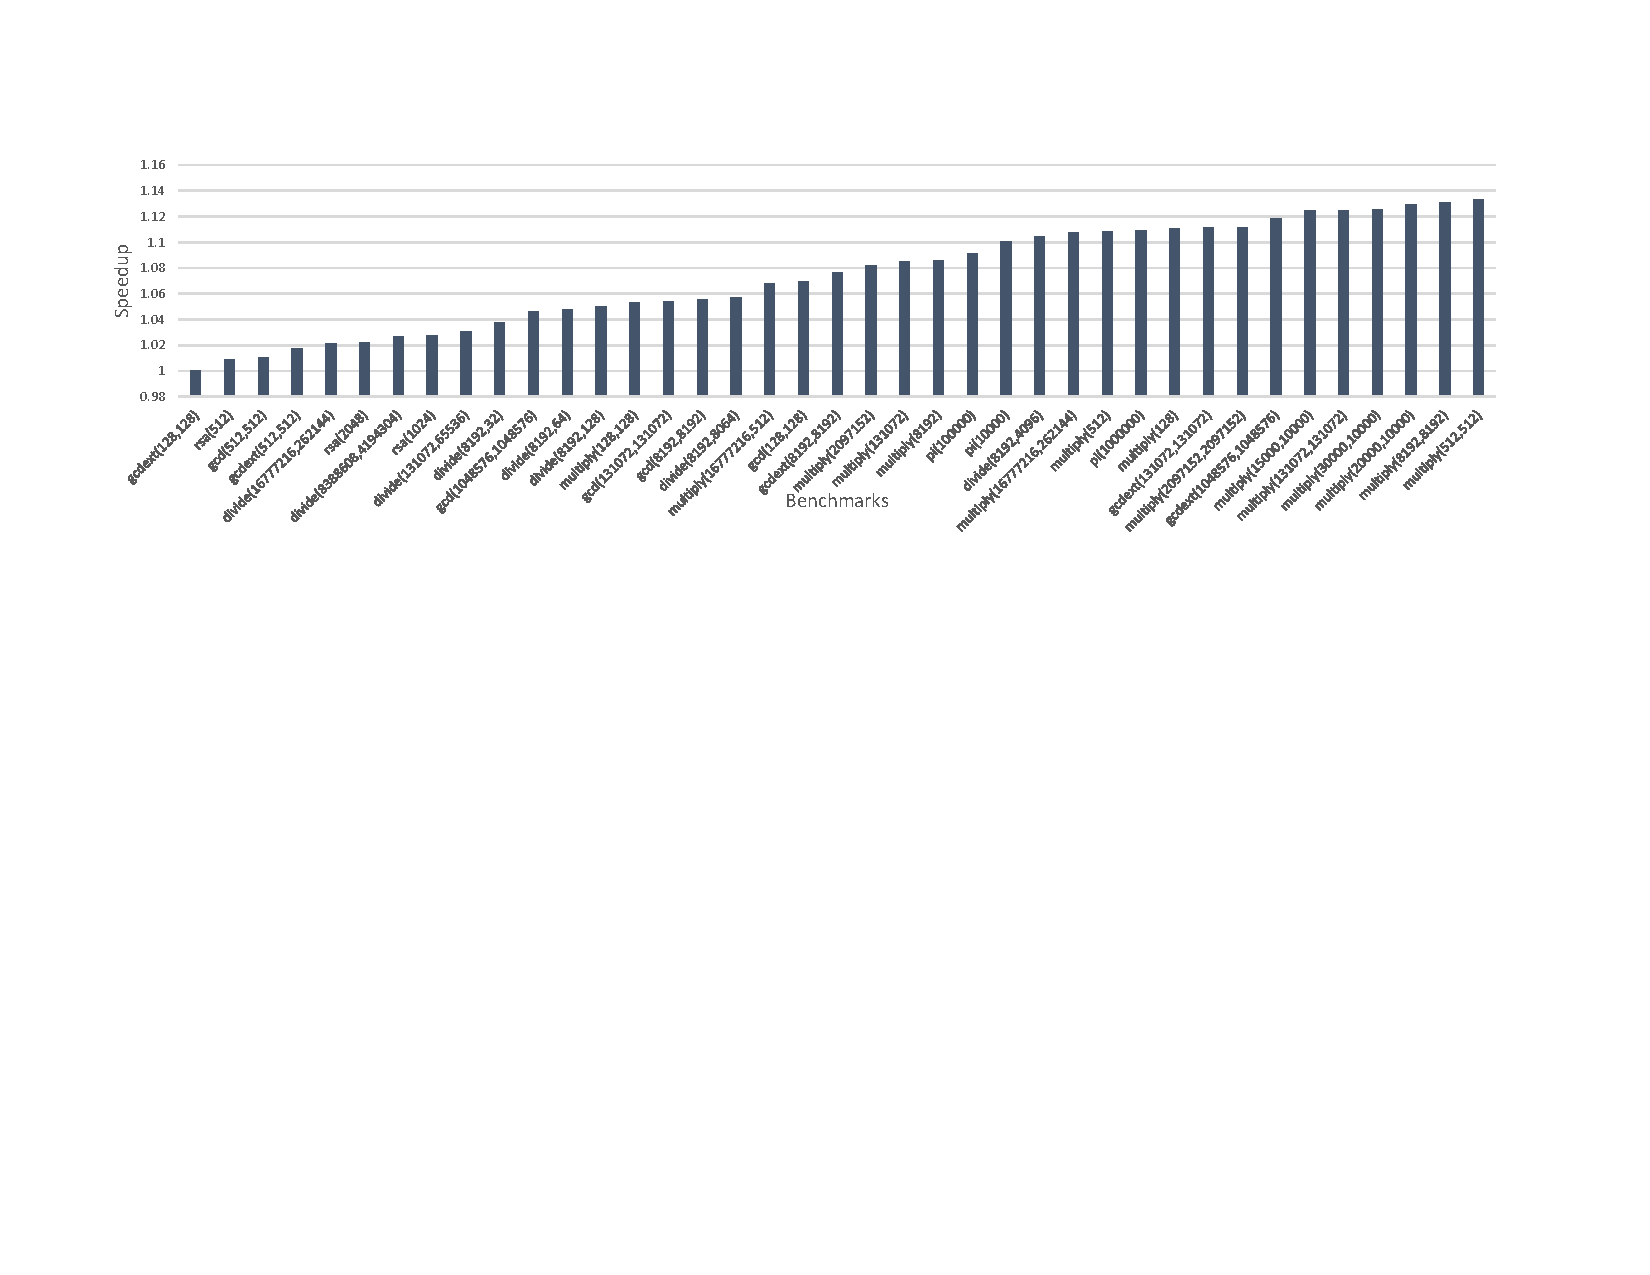
\includegraphics[page=1,width=\linewidth]{figures/data.pdf}
%   }`
%   \hfill'
%   \subfloat[Targeting AMD Zen 3; geomean=1.021x\label{plot:loops-amd}]{
%     \includegraphics[page=2,width=\linewidth]{figures/data.pdf}
%   }
%   \caption{Speedups---estimated by LLVM-MCA---due to running \minotaur{}
%     on a loop micro-benchmark suite}
% \end{figure*}

It is important for \minotaur{} to extract cuts that are of an appropriate
size.
%
If they are too large, compile times suffer and also the SMT solver
can be overwhelmed, leading to timeouts; if cuts are too small, then
they form an insufficient basis for driving an optimization.
%
To determine a good value for $B$, the depth parameter to the cut
extraction procedure shown in Algorithm~\ref{alg:slicing}, we
performed an empirical study.
%
We started with FlexC's benchmark suite~\cite{woodruff2023rewriting},
a collection of 2,386 compilable, non-trivial C functions containing
loops from FFMPEG, FreeImage, DarkNet, xz, bzip2, and the LivermoreC
benchmark.
% \footnote{The loop data set was provided
% by Alexander Brauckmann and Michael O'Boyle at the University of
% Edinburgh, UK\@.  At present, no citable reference for this work
% exists.}
%
When compiled to LLVM IR, these functions contain a total of 123,062
instructions; thus, our cut extractor was invoked 123,062 times for
each depth bound.
%
We chose this code as the basis for our experiment because it is
derived from real applications while also being small enough to
keep compile times manageable (compared to, e.g., SPEC CPU 2017,
which is much larger).


\begin{figure}[tbp]
  \centering
  \subfloat[Unique cuts extracted\label{fig:loop-expression}]{
    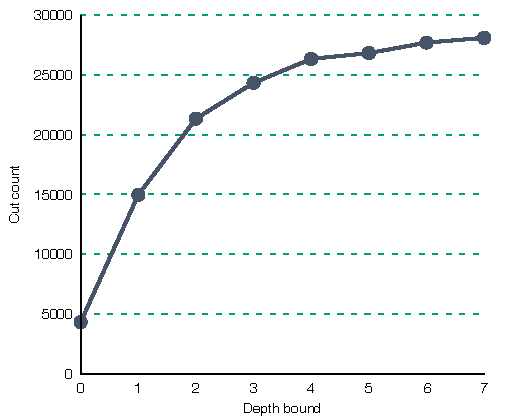
\includegraphics[width=0.32\linewidth]{figures/spec/expression-count.pdf}
  }
  \hfill
  \subfloat[Unique opts. synthesized\label{fig:loop-optimization}]{
    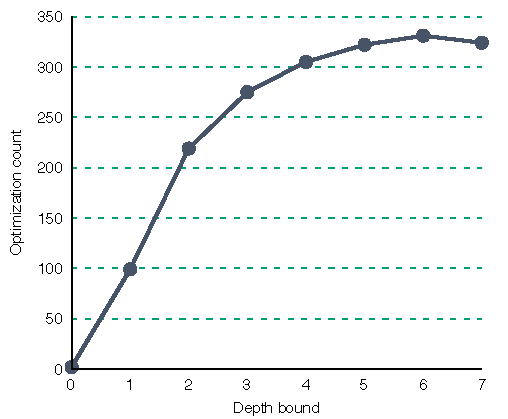
\includegraphics[width=0.32\linewidth]{figures/spec/optimization-count.pdf}
  }
  \hfill
  \subfloat[Compilation time\label{fig:loop-buildtime}]{
    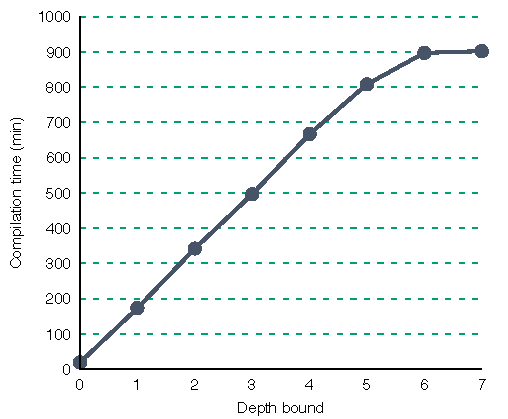
\includegraphics[width=0.32\linewidth]{figures/spec/compilation-time.pdf}
  }
  \caption{Evaluating the effect of varying $B$, the depth bound for
    cut extraction}
  \label{fig:loop}
\end{figure}


We then ran \minotaur{} on these functions with all depth bounds from
0--7, measuring the number of unique cuts that were extracted, the
number of optimizations found, and the compilation time.
%
We used a one-minute timeout for individual Z3 queries, and we also
gave \minotaur{} a total of up to five minutes to synthesize an optimized
version of each cut.
%
Figure~\ref{fig:loop} summarizes the results of this experiment.
%
The number of unique cuts that are extracted grows quickly with $B$,
but eventually begins to saturate simply because the functions being
compiled do not always have very long dependency chains.
%
The number of synthesized optimizations also grows quickly, but it
peaks when $B=6$ and then it decreases because the size of the cuts
causes many solver timeouts.
%
Finally, the total compile time increases smoothly with the depth
bound, eventually leveling off as most solver queries time out.


For the experiments in the rest of the evaluation section, we chose
$B=4$ because this gets pretty close to the maximum observed number of
optimizations without requiring exorbitant compile times.
%
It seems likely that there is room for improvement in this aspect of
\minotaur: perhaps the depth bound should be determined adaptively.
%
In this scenario, we would extract more and more components into the
cut, until either an optimization is found or else the solver begins
to time out.
%
We leave explorations of this nature for future work.


\subsection{Speedups for Benchmarks and Applications}

In this section, we show how \minotaur{} speeds up real-world benchmarks
and applications.

\paragraph{Experimental setup}
%
We used two machines for our evaluation: one with an Intel Xeon Gold
6210U processor running at 2.5\,GHz (this implements the Cascade Lake
microarchitecture~\cite{cascadelake}) and the other with an
AMD Ryzen 5950x processor
running at 3.4\,GHz (this implements the Zen~3 microarchitecture~\cite{zen3}).
The Intel machine supports the AVX-512 instruction set.
%
Both machines run Linux and were idle except for a single core running
our benchmarks.
%
To reduce the performance variation caused by frequency scaling, we
disabled turbo boost on the Intel machine and the core performance
boost on the AMD machine.
%
We invoked LLVM with the \texttt{-march=native} compilation flag to
ask it to take maximum advantage of processor features; we left other
compilation flags unchanged, except where noted.
%
All benchmarks are compiled at the \texttt{-O3} optimization level.
%
We set the timeout for Z3~\cite{z3} queries to one minute.
%
Finally, for each instruction that it tries to optimize, \minotaur{} gives
up if no solution is found within five minutes.


\paragraph{Benchmark selection}
%
We evaluate on SPEC CPU 2017%\footnote{\url{https://www.spec.org/cpu2017/}}
because it is a widely accepted standard
benchmark.
%
We only evaluate on the \emph{speed} subset of the SPEC suite, and we omit
648.exchange, 607.cactuBSSN, 621.wrf, 627.cam4, 628.pop2, 649.fotonik3d,
and 654.roms as they contain Fortran code.
%
We additionally use GMP, the GNU Multiple Precision Library, and libYUV,
which is used by Google Chrome/Chromium for manipulating images in the
YUV format.
%
We chose these libraries because they have been heavily tuned for
performance, they rely on loops, and they come with performance
benchmark suites that we could simply reuse.


\paragraph{Compile times}
%
Table~\ref{tab:compiletime} shows how long it takes \minotaur{} to process
our benchmarks, along with the number of potentially optimizable
values and the number of optimizations found.
%
In most cases, \minotaur{} found more optimizations when targeting the AMD
processor.
%
We believe this is because LLVM is more mature targeting
AVX2 than AVX512.
%
Solving queries with 256-bit vectors is also less likely to cause Z3
to timeout than are 512-bit vectors.
%
Minotaur is quite slow when it runs with a cold cache because it
performs a large number of solver queries.
%
However, with a warm cache, it is only 3\% slower than baseline \texttt{clang}.

\begin{table}[t]
  \centering
  \begin{tabular}{| r | r r  r | r r | r r r | r r |}
    \hline
    \multirow{2}{*}{}& \multicolumn{5}{c|}{Intel Cascade Lake} & \multicolumn{5}{c|}{AMD Zen3} \\
    \cline{2-11}
    & \multicolumn{3}{c|}{Compilation time (min)} & \multicolumn{2}{c|}{Opt. found} & \multicolumn{3}{c|}{Compilation time (min)} & \multicolumn{2}{c|}{Opt. found}  \\
    \hline
    Benchmarks & cold cache & warm & clang & \# cut & \# opt. & cold cache & warm & clang & \# cut & \# opt. \\
    \hline\hline
    SPEC CPU 2017 & 2,337 & 3 & 3 & 109,177 & 2,683 & 2,580 & 3 & 3 & 114,612 & 2,820 \\
    \hline
    gmp-6.2.1 & 440 & < 1 & < 1 & 9,170 & 336 & 445 & < 1 & < 1 & 9,265 & 387\\
    \hline
    libYUV & 2,196 & < 1 & < 1 & 6,849 & 334  & 2,193 & < 1 & < 1 & 6,809 & 357 \\
    % \hline
    % OpenBLAS-0.3.26 & 554 & < 1 & < 1 & 8,683 &  & 670 & < 1 & < 1 & 9,182 & 156 \\
    \hline
  \end{tabular}
  \caption{Compile-time statistics}
  \label{tab:compiletime}
\end{table}

\paragraph{Optimizing GMP with \minotaur{}}

\begin{figure}[tbp]
  \centering
  \subfloat[Speedups on Intel Cascade Lake, geomean = 1.073x\label{plot:gmp-intel}]{
    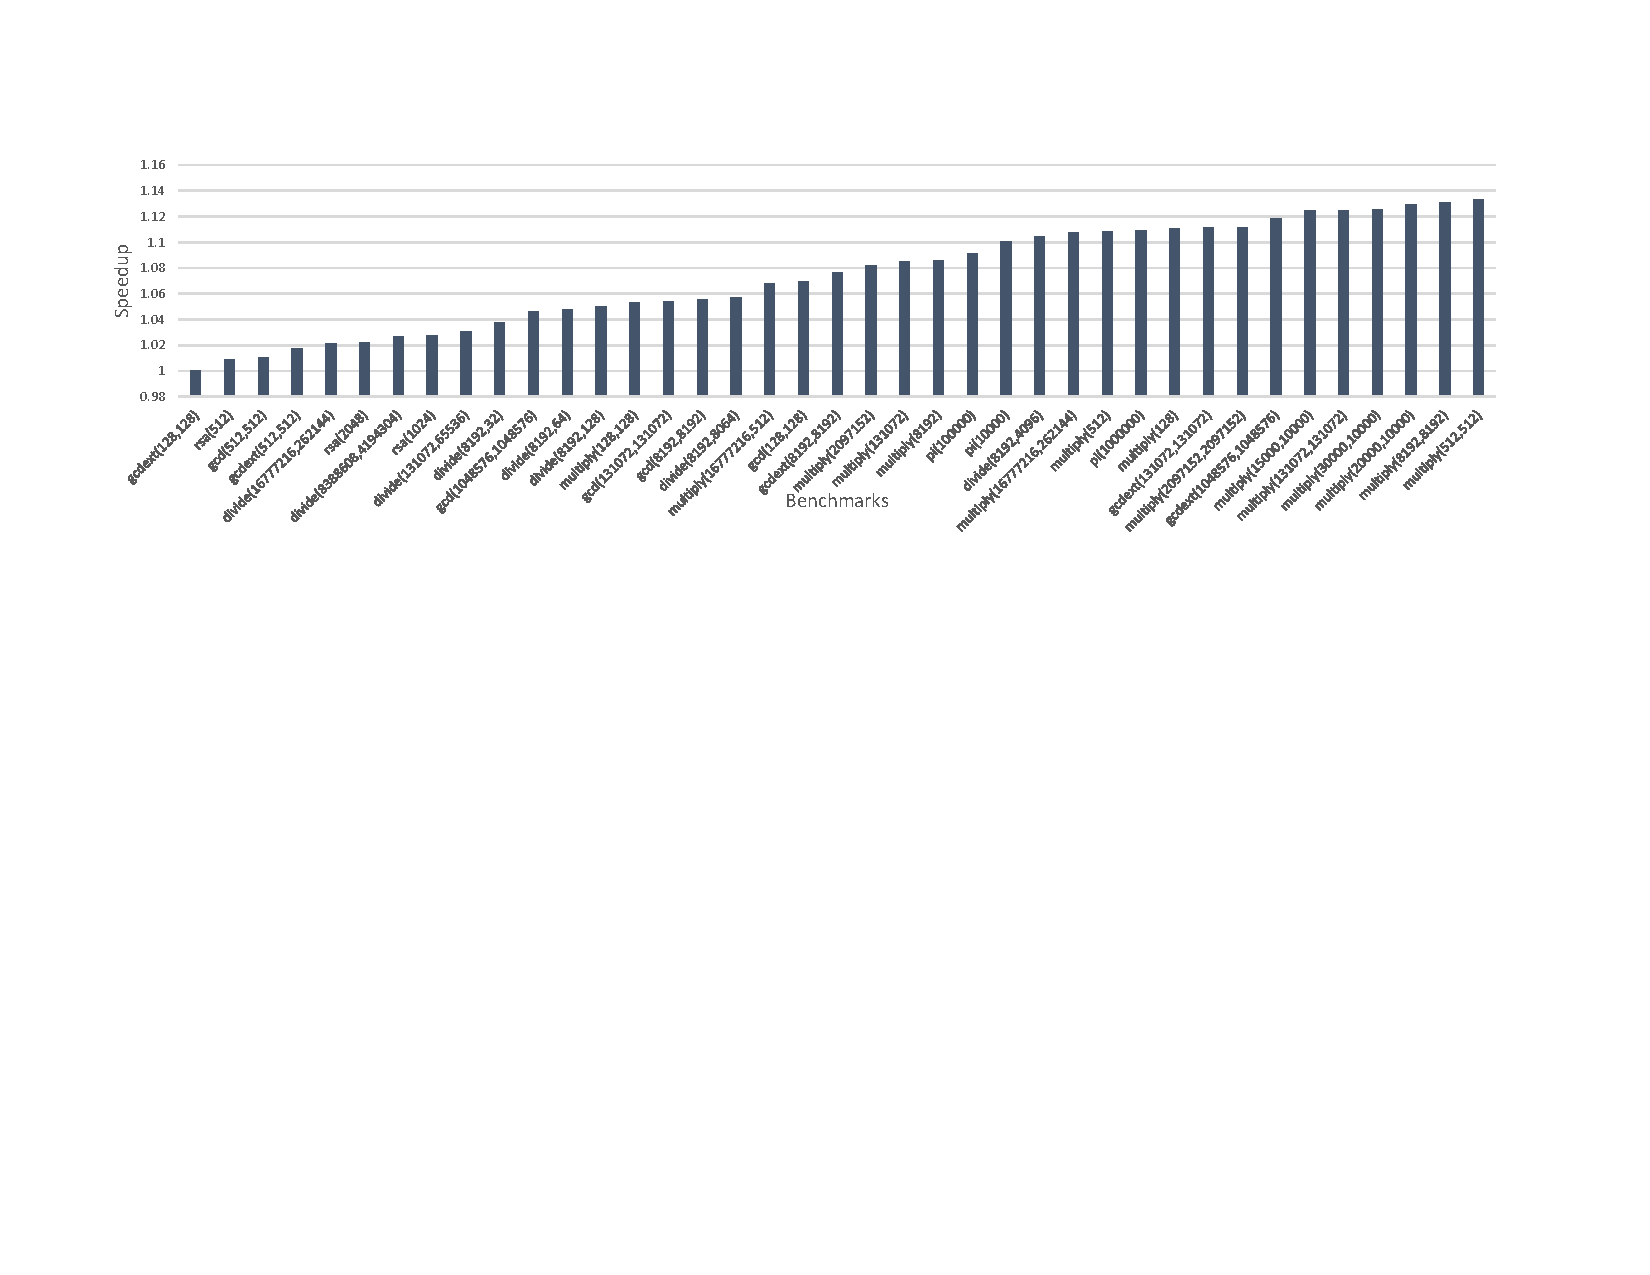
\includegraphics[page=1,width=\linewidth]{figures/data.pdf}
  }
  \hfill
  \subfloat[Speedups on AMD Zen 3, geomean = 1.065x\label{plot:gmp-amd}]{
    \includegraphics[page=2,width=\linewidth]{figures/data.pdf}
  }
  \caption{GNU Multiple Precision Library (GMP) speedups}
  \label{fig:gmp}
\end{figure}


GMP provides a portable C-language implementation and then, for
several platforms, a faster assembly language implementation.
%
For this evaluation, we selected the C implementation, because \minotaur{}
works on LLVM IR and cannot process assembly code at all.
%
The benchmark suite that we used is
GMPbench.%\footnote{\url{https://gmplib.org/gmpbench}}
%
Figure~\ref{fig:gmp} summarizes the results.
%
When \minotaur{} targets the Intel Cascade Lake processor, and when the
resulting executables are run on that same microarchitecture,
all the benchmarks sped up;
across all of the benchmarks, the mean speedup was 7.3\%.
%
The analogous experiment using the AMD Zen~3 microarchitecture
resulted in one benchmark slowing down, and the rest of benchmarks
speeding up, for an overall mean speedup of 6.5\%.


\paragraph{Optimizing libYUV with \minotaur{}}

\begin{figure}[tbp]
  \centering
  \subfloat[Speedups on Intel Cascade Lake, geomean = 1.022x\label{plot:libyuv-intel}]{
    \includegraphics[page=3,width=\linewidth]{figures/data.pdf}
  }
  \hfill
  \subfloat[Speedups on AMD Zen 3, geomean = 1.029x\label{plot:libyuv-amd}]{
    \includegraphics[page=4,width=\linewidth]{figures/data.pdf}
  }
  \caption{LibYUV speedups}
  \label{fig:yuv}
\end{figure}


This library has an extensive test suite, part of which is explicitly
intended for performance testing; we used this part as a benchmark.
%
Each of them scales, rotates, or converts a 1280\,x\,728 pixel
image 1,000 times.
%
Figure~\ref{fig:yuv} shows the results of this experiment.
%
When \minotaur{} targets an Intel processor, $148$ programs slowed down, $72$
did not change performance, and $2,312$ sped up, for an overall speedup of
2.2\%.
%
Targeting an AMD processor, $188$ programs slowed down, $85$ did not
change performance, and $2,259$ sped up, for an overall speedup of 2.9\%.
%
\minotaur{} can make code slower because it looks at optimizations in
isolation; it does not attempt to model interactions between
optimizations.


libYUV is portable code, but it has already been heavily tuned for
performance; most commits to its repository over the last several
years have been performance-related.
%
Our hypothesis is that this manual tuning has already eaten up most of
the performance gains that we would have hoped to gain from \minotaur{}.
%
For some time now, Google's released versions of Chrome have been
compiled using LLVM; the Chrome engineers have had ample time to
ensure that this compiler achieves decent code generation for
performance-critical libraries.

% \begin{figure*}[tbp]
%   \centering
%   \subfloat[Normalized speedup; geomean = 1.013x\label{fig:spec-intel-speed-ups}]{
%     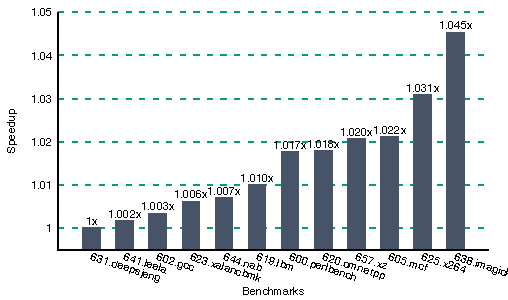
\includegraphics[width=0.45\linewidth]{figures/spec/spec-intel.pdf}
%   }
%   \hfill
%   \subfloat[Compilation time in seconds\label{fig:spec-intel-compilation-time}]{
%     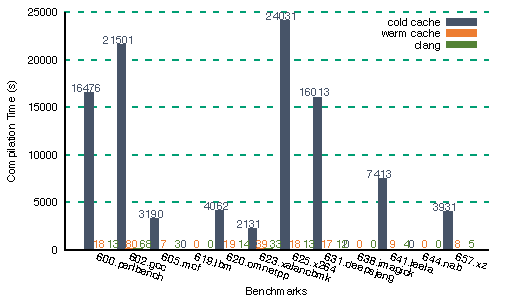
\includegraphics[width=0.45\linewidth]{figures/spec/spec-intel-compiletime.pdf}
%   }
%   \caption*{Targeting Intel Cascade Lake\label{fig:spec-intel}}
%   \hfill
%   \subfloat[Normalized speedup; geomean = 1.012x\label{fig:spec-amd-speed-ups}]{
%     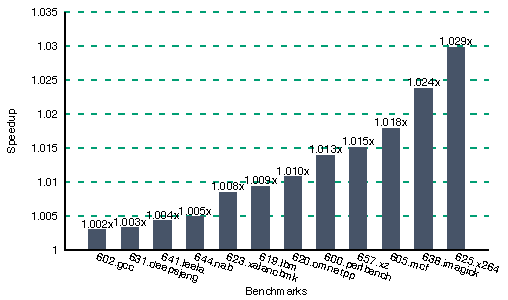
\includegraphics[width=0.45\linewidth]{figures/spec/spec-amd.pdf}
%   }
%   \hfill
%   \subfloat[Compilation time in seconds\label{fig:spec-amd-compilation-time}]{
%     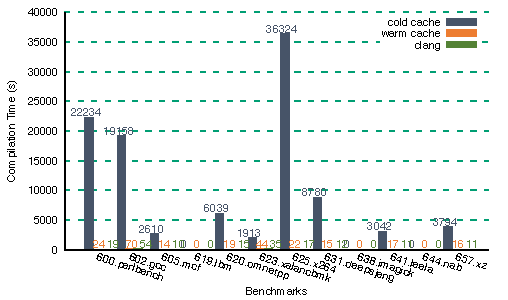
\includegraphics[width=0.45\linewidth]{figures/spec/spec-amd-compiletime.pdf}
%   }
%   \caption*{Targeting AMD Zen 3\label{fig:spec-amd}}
%   \caption{SPEC CPU2017 benchmark performance and compilation time}
%   \label{fig:spec}
% \end{figure*}

\begin{figure}[tbp]
  \centering
  \subfloat[Speedups on Cascade Lake; geomean = 1.015x\label{fig:spec-intel-speed-ups}]{
    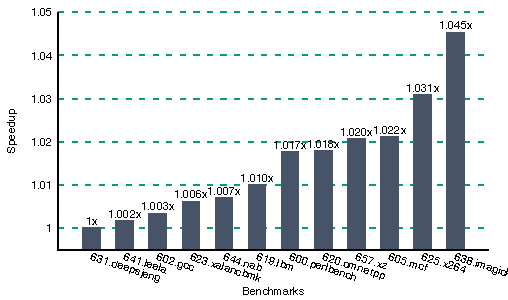
\includegraphics[width=0.48\linewidth]{figures/spec/spec-intel.pdf}
  }
  \hfill
  \subfloat[Speedups on Zen 3; geomean = 1.012x\label{fig:spec-amd-speed-ups}]{
    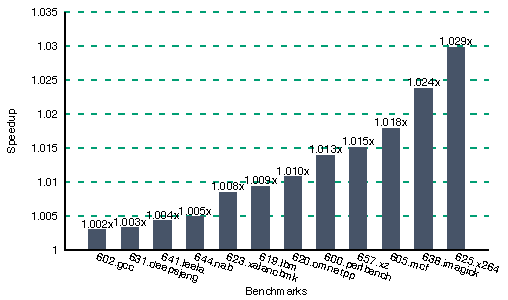
\includegraphics[width=0.48\linewidth]{figures/spec/spec-amd.pdf}
  }
  \caption{SPEC CPU2017 benchmark performance}
  \label{fig:spec}
\end{figure}

\paragraph{Optimizing SPEC CPU2017 with \minotaur{}}

Figure~\ref{fig:spec} shows the effect of optimizing the benchmarks
from SPEC CPU2017 using \minotaur.
%
When optimizing for, and running on, the Intel processor, we observed
a mean speedup of 1.5\%.
%
When optimizing for, and running on, the AMD processor, we observed a
mean speedup of 1.2\%.
%
It is notoriously difficult to speed up the SPEC CPU benchmarks
because compiler engineers have already put considerable effort into
achieving good code generation for them.



\subsection{Optimizations Discovered by \minotaur}
\label{sec:examples}

The purpose of this section is to examine \minotaur's strengths by
presenting some optimizations that it found while compiling benchmark
programs.
%
None of these optimizations can be performed by the version of LLVM
that \minotaur{} is based on,
%\footnote{\minotaur{} uses LLVM~18.1.0 for all results in this paper.}
at its \texttt{-O3} optimization level.
%
We present optimizations in an SSA format that is close to LLVM IR,
but we have edited it slightly for compactness and legibility.

\iffalse
One might be inclined to ask, while reading this section, ``Why is
LLVM incapable of performing this transformation?''
%
Alas, there is no single answer.
%
In some cases, performing the transformation would require the
optimizer to have a semantic model of a processor-specific intrinsic
function, but mostly these models do not exist.
%
In other cases, such as Example~5 below, generic reasoning about the
code would be very difficult, and a specific pattern matcher might not
be robust enough to be worth implementing.
%
Finally, our observation is that vector support in LLVM is somewhat
newer and less mature than support for other IR features, and the
optimizers have simply not had enough time to accumulate the requisite
optimizations.
\fi


\paragraph*{Example 1}

This code is from perlbench in SPEC:

{\small\begin{quote}\begin{verbatim}
%0 = zext <16 x i8> %x to <16 x i16>
%1 = zext <16 x i8> %y to <16 x i16>
%2 = call @llvm.x86.avx2.pavg.w(%0, %1)
%3 = trunc <16 x i16> %2 to <16 x i8>
ret <16 x i8> %3
  =>
%0 = call @llvm.x86.sse2.pavg.b(%x, %y)
ret <16 x i8> %0
\end{verbatim}
\end{quote}}

The unoptimized code zero-extends each 8-bit element of the two input
vectors to 16~bits, calls the AVX2 variant of \texttt{pavg} to perform
element-wise averaging of the extended vectors, and then truncates
elements of the resulting vector back to eight bits.
%
The optimized code simply calls an SSE2 version of the \texttt{pavg}
instruction that operates on 8-bit elements, reducing the uOp cost
of the operation from four to one.


\paragraph*{Example 2}
%https://godbolt.org/z/vjjr7MGzb

This code is from libYUV, ``... an open source project that includes
YUV scaling and conversion
functionality'':
%m\footnote{\url{https://chromium.googlesource.com/libyuv/libyuv/}}

{\small\begin{quote}\begin{verbatim}
%0 = call @llvm.x86.avx2.pmadd.wd(%x, <0,1,0,1, ...>)
%1 = call @llvm.x86.avx2.pmadd.wd(%x, <1,0,1,0, ...>)
%2 = sub nsw <8 x i32> %1, %0
ret <8 x i32> %2
  =>
%0 = call @llvm.x86.avx2.pmadd.wd(%x,<1,-1,1,-1, ...>)
ret <8 x i32> %0
\end{verbatim}
\end{quote}}

The \texttt{pmadd.wd} (multiply and add packed integers) instruction multiplies
signed 16-bit integers element-wise from two input vectors, and then
computes its output by adding adjacent pairs of elements from the
resulting vector.
%
Thus, the input to this instruction is two 16-way vectors containing
16-bit elements, and its output is a single 8-way vector of 32-bit
elements.


In this example, the second argument to each \texttt{pmadd.wd}
instruction in the unoptimized code is a vector of alternating zeroes
and ones, which has the effect of selecting odd-indexed elements into
\texttt{\%0} and even-indexed elements into \texttt{\%1}.
%
Then, after the \texttt{sub} instruction, which simply performs
element-wise subtraction of \texttt{\%0} and \texttt{\%1}, the overall
effect of this code is to compute the difference between adjacent
pairs of elements of \texttt{\%x}.
%
\minotaur{} is able to perform this same computation using a single
\texttt{pmadd.wd} instruction which negates odd-numbered elements of
\texttt{\%x} before performing the addition.
%
The optimized code requires $5$ uOps to execute whereas the original
code requires $8$.


\paragraph*{Example 3}

This code is from libYUV:

%https://godbolt.org/z/7ooobqofK
{\small\begin{quote}\begin{verbatim}
%0 = shufflevector <32 x i8> %x, poison, <3, 7, 11, 15, 19, 23, 27, 31>
%1 = lshr %0, <6, 6, 6, 6, 6, 6, 6, 6>
%2 = zext 8 x i8> %1 to <8 x i32>
ret <8 x i32> %2
  =>
%0 = bitcast <32 x i8> %x to <8 x i32>
%1 = call @llvm.x86.avx2.psrli.d(<8 x i32> %0, 30)
ret <8 x i32> %1
\end{verbatim}
\end{quote}}

The \texttt{shufflevector} instruction in the unoptimized code selects
every fourth byte-sized element from the input \texttt{\%x}.
%
The resulting 8-way vector is right-shifted element-wise by six bit
positions, and that result is zero-extended to an 8-way vector of
32-bit elements.
%
\minotaur's optimized version (which executes in 4 uOps instead of 11)
first reinterprets the input vector's data as 32-bit elements; this
bitcast is relevant to LLVM's type system, but it is a nop at the CPU
level.
%
Then, the \texttt{prsli} instruction shifts each 32-bit element to the
right by 30 bit positions.
%
This right-shift-by-30 achieves the same effect as the unoptimized
code, where the \texttt{shufflevector} can be seen as a
right-shift-by-24, followed by an explicit right-shift-by-6.

\paragraph*{Example 4}

This code, from compiling perlbench from SPEC CPU 2017, illustrates
\minotaur's ability to reason about control flow:

% control flow divergence
%https://godbolt.org/z/e8jTsTMMz
{\small\begin{quote}\begin{verbatim}
entry:
  br i1 %c, label %body, label %if.end
body:
  br label %if.end
if.end:
  %p1 = phi [ %a, %body ], [ %b, %entry ]
  %p2 = phi [ %b, %body ], [ %a, %entry ]
  %r = call @llvm.x86.avx2.pavg.b(%p1, %p2)
  ret <32 x i8> %r
    =>
  %r = call @llvm.x86.avx2.pavg.b(%a, %b)
  ret <32 x i8> %r
\end{verbatim}
\end{quote}}

The intent of the code is to compute the element-wise average of input
vectors \texttt{\%a} and \texttt{\%b}, with a Boolean value
\texttt{\%c} determining the order in which the input vectors are
presented to the \texttt{pavg} instruction.
%
However, the order of arguments to this instruction does not matter, and
\minotaur's version executes in 4 uOps while the original code requires
10.
%
Note that \minotaur{} was not explicitly taught that \texttt{pavg} is
commutative; the necessary information was inferred naturally from the
formal specification.


\paragraph*{Example 5}

This is an optimization discovered
by \minotaur{} when it was used to compile GMP, the GNU Multiple Precision
Arithmetic Library, a widely-used library for arbitrary precision
integer computation:
%q\footnote{\url{https://gmplib.org/}}

% before 19 after 13

{\small\begin{quote}\begin{verbatim}
%0 = lshr i64 %x, 1
%1 = and i64 %0, 0x5555555555555555
%2 = sub i64 %x, %1
%3 = lshr i64 %2, 2
%4 = and i64 %2, 0x3333333333333333
%5 = and i64 %3, 0x3333333333333333
%6 = add nuw nsw i64 %4, %3
%7 = lshr i64 %6, 4
%8 = add nuw nsw i64 %7, %6
%9 = and i64 %8, 0xf0f0f0f0f0f0f0f
ret i64 %9
  =>
%0 = bitcast i64 %x to <8 x i8>
%1 = call @llvm.ctpop(<8 x i8> %0)
%2 = bitcast <8 x i8> %1 to i64
ret i64 %2
\end{verbatim}
\end{quote}}

%
% \vspace{0.1in}
% %
% \caption{On the left, LLVM IR extracted from GMP; when compiled to
%   x86-64 code and run on an Intel Cascade Lake processor, its
%   predicted execution cost is 19 uOps. On the right, \minotaur's
%   optimized version of this code, which requires 13 uOps on the same
%   target.}
% \label{fig:ctpop}
% \end{figure*}
%
The original code performs a series of bit-level
manipulations on a 64-bit integer value, with the net result of
performing an 8-way vectorized 8-bit popcount operation.\footnote{The
popcount, or Hamming weight, of a bitvector is the number of ``1''
bits in it.}
%
The optimized code simply calls an intrinsic function to do the
popcount; it costs 13 uOps instead of the original code's 19.
%
Although robust recognition of open-coded idioms is not the focus
of our work, \minotaur{} does sometimes manage to achieve this.

Taking a strict view of types in the synthesis process could help
prune the search space, but it would also cause us to miss
optimizations that require a flexible view of types.
%
This example illustrates the latter case: the original code contains
no indication that a good optimization can be found using a vector of
type <8 x i8>, and therefore a strictly type-guided synthesis
procedure would miss this one.

\paragraph*{Example 6}

This code comes from 644.nab in SPEC CPU 2017:

% https://github.com/llvm/llvm-project/issues/85250
{\small\begin{quote}\begin{verbatim}
%0 = fcmp oge float %x, 0.000000e+00
%1 = fneg float %x
%2 = select i1 %0, float %0, float %2
%3 = fcmp oeq float %2, 0.000000e+00
ret i1 %3
  =>
%1 = fcmp oeq float %x, 0.000000e+00
ret i1 %oeq
\end{verbatim}
\end{quote}}

The original code computes the absolute value of a floating-point
number \texttt{\%x} and then checks if the result is zero.
\minotaur{} found that that the original code is equivalent to simply checking if
\texttt{\%x} is zero.


\paragraph*{Example 7}

This code is from the SPEC CPU 2017 benchmark 619.lbm:

% https://github.com/llvm/llvm-project/issues/85245
{\small\begin{quote}\begin{verbatim}
%0 = fsub float %x, %y
%1 = fcmp ogt float %0, 0.000000e+00
ret i1 %3
  =>
%0 = fcmp ogt float %x, %y
ret i1 %0
\end{verbatim}
\end{quote}}

The original code computes the difference between two floating-point
values, and then checks if the result is greater than zero. \minotaur{}
found that this code is equivalent to checking if the second value is
less than the first.


\paragraph*{Example 8}

This code comes from 619.lbm in SPEC CPU 2017:

% https://github.com/llvm/llvm-project/issues/85267

{\small\begin{quote}\begin{verbatim}
%0 = fmul float %x, 0x3FF0CCCCC0000000
%1 = fcmp olt float %t1, 0x3FE20418A0000000
ret i1 %1
  =>
%0 = fcmp ole float %x, 0x3FE12878E0000000
ret i1 %0
\end{verbatim}
\end{quote}}

The original code multiplies a floating-point value \texttt{\%x} by a
constant, and then checks if the result is less than another constant.
\minotaur{} found that this code is equivalent to checking if \texttt{\%x}
is less than or equal to a third constant.
It is tricky to reason about floating-point literals, and \minotaur{} is able to
reason and synthesize the correct literals correctly.

\paragraph*{Example 9}

This code comes from 638.imagick in SPEC CPU 2017:

{\small\begin{quote}\begin{verbatim}
%0 = fmul float %x, 0.000000e+00
%1 = fmul float %0, 3.000000e+00
ret float %1
  =>
%0 = fmul float %x, 0.000000e+00
ret i1 %0
\end{verbatim}
\end{quote}}

The original code multiplies a floating-point value \texttt{\%x} by
zero, and then multiplies the result by 3.0. \minotaur{} found that this
code is equivalent to multiplying \texttt{\%x} by zero directly.
Note the original code cannot be optimized to 0.0 directly, because of
the NaN and signed zero propagation rules in floating-point arithmetic.
This example shows that \minotaur{} is able to reason about these corner
cases and synthesize the correct code.

% \paragraph*{Example 10}


%TODO: Add one final example
% place holder for a good example





\section{Related Work}

A \emph{superoptimizer} is a program optimizer that meaningfully
relies on search to generate better code, in contrast with traditional
compilers that attempt a fixed (but perhaps very large) sequence of
transformations.
%
The eponymous superoptimizer~\cite{massalin} exhaustively generated
machine instruction sequences, using various strategies to prune the
search space, and using testing to weed out infeasible candidates.
%
Also predating modern solver-based methods, Davidson and Fraser~\cite{peep84}
constructed peephole optimizations from machine description files.
%
In contrast, modern superoptimizers rely on solvers to perform
automated reasoning about program semantics.


Souper~\cite{souper} is a synthesizing superoptimizer that works on
LLVM IR; it is the most directly connected previous work to \minotaur{}.
%
Souper's slicing strategy is similar to \minotaur's in that it extracts a
DAG of LLVM instructions that overapproximates how a given SSA value
is computed.
%
However, unlike Souper, \minotaur{} extracts memory operations and
multiple basic blocks, so it is capable of (we believe) strictly more
transformations than Souper is able to perform.
%
Additionally, Souper's undefined behavior model does not capture all
of the subtleties of undefined behavior in LLVM, whereas we reuse
Alive2's model, which is probably the most widely used formalization
of these semantics, and is generally recognized as being correct.
%
Finally, \minotaur{} focuses on vector-related transformations, whereas
Souper supports neither LLVM's portable vector instruction set nor its
platform-specific intrinsics.


\minotaur{} is also strongly inspired by Bansal and Aiken's
work~\cite{Bansal06}; their superoptimizer operated on x86 assembly
code and was able to make interesting use of vector instructions.
%
Starting from unoptimized assembly produced by GCC, it was able to
produce code competitive with higher optimization levels.
%
The overall structure of this superoptimizer, where program slices
are extracted, canonicalized, checked against a cache, and then
optimized in the case of a cache miss, is very similar to \minotaur{}, but
there are many differences in the details, particularly in \minotaur's
slice extractor which allows its synthesis specification to
approximate the original code's effect much more closely.
%
Another assembly superoptimizer, STOKE~\cite{stoke,stoke-fp,conditionally},
is not as closely related; it is based on randomly
perturbing assembly-language functions.
%
STOKE can potentially perform transformations that Minotaur cannot,
but we believe that its results are more difficult to translate into
standard peephole optimizations than are Minotaur's.


Several recent projects have focused not on optimizing individual
programs but rather on generating program rewrite rules.
%
OptGen~\cite{optgen} finds scalar peephole optimizations that meet
a specified syntactic form.
%
Even at small rewrite sizes, it was able to find numerous
optimizations that were missing from the 2015 versions of GCC and
LLVM\@.
%
VeGen~\cite{vegen} generates SLP vectorization rules---an SLP
vectorizer~\cite{slp} merges a set of scalar operations into vector
instructions.
%
VeGen parses the Intel Intrinsics Guide~\cite{intelguide} and uses this
to build pattern matchers for x86 vector instructions.
%
VeGen applies the pattern matchers to an input scalar program, and
replaces scalar expressions with vector instructions when it
finds a profitable match.
%
VeGen uses syntactic pattern matching rather than solver-based
equivalence/refinement checking.
%
Diospyros~\cite{diospyros} is another vector rewrite rule generator,
it takes an equality saturation~\cite{equalitysat} approach and uses a translation
validator to reject unsuitable candidates.
As an equality saturation-based tool, Diospyros builds its search space
with existing rewrite rules.


Program synthesis---generating implementations that conform to
a given specification---is intimately related to superoptimization.
%
Rake~\cite{rake} performs instruction selection for vectorized
Halide~\cite{halide} expressions using a two stage synthesis
algorithm.
%
First, Rake synthesizes a data-movement-free sketch~\cite{sketch}, and
then in the second stage it concretizes data movement for the
sketch via another synthesis query.
%
Rake targets Hexagon DSP processors~\cite{hexagon} which share some functionally
similar SIMD instructions with x86\@.
%
Cowan et al.~\cite{ml_syn} synthesized quantized machine learning
kernels.
%
Their work introduces two sketches: a compute sketch, which computes a matrix
multiplication, and a reduction sketch that collects the computation
result to the correct registers.
%
It relies on Rosette~\cite{rosette} to generate an efficient NEON~\cite{neon}
implementation that satisfies the specifications for those two
sketches.
%
Swizzle Inventor~\cite{swizzleinventor} is another tool built on
Rosette; it synthesizes data movement instructions for a GPU compute
kernel, and it requires user-defined sketches describing the
non-swizzle part of the program.
%
MACVETH~\cite{sparse} generates high-performance vector packings of
regular strided-access loops, by searching for a SIMD expression that
is equivalent to a gather specification.
%
All of these works show good performance results, but they focus on
relatively narrow tasks, whereas \minotaur{} attempts to improve SIMD
programs in general.


Most previous superoptimizers and program synthesizers use simple
cost models.
%
For example, Souper~\cite{souper} assigns each kind of instruction a
weight and uses the weighted sum as the cost of a rewrite.
%
This kind of cost model is not a very good predictor of performance
on a modern out-of-order processor.
%
\minotaur{} and MACVETH~\cite{sparse} use the LLVM-MCA~\cite{llvmmca}
microarchitectural performance analyzer, which can still lead to
mispredictions, but it is generally more accurate than simple
approaches are.

\chapter{Conclusion}
\label{chap:conclusion}

This section concludes the thesis by summarizing the contributions.
%
The work established in this thesis is done on two different optimization
domains: peephole generation and collective communication synthesis.
%
The thesis that this dissertation has supported is that program synthesis can
be used to generate optimized and verifiable code for novel architectures.


This dissertation introduced \minotaur{}, a SIMD-oriented
superoptimizer that automatically
 generates peephole optimizations for LLVM IR code.
%
\minotaur{} has been shown to discover optimizations that are missed by
commodity compilers, and has demonstrated speedups on a variety of
benchmarks.

This dissertation also proposed SCCL, a syntheizer that generates
optimal collective communication algorithms a given hardware topology.
%
SCCL synthesizes algorithms along the Pareto-frontier spanning from
latency-optimal to bandwidth-optimal implementations of a collective.
%
The algorithm generated by SCCL are competitive with hand-optimized
collective communication libraries.


I hope that this work will inspire future research in the area of program
synthesis for performance optimization.


%%
%% The next two lines define the bibliography style to be used, and
%% the bibliography file.
\bibliographystyle{ACM-Reference-Format}
\bibliography{references}


%%
%% If your work has an appendix, this is the place to put it.
\appendix
\section{Artifact Appendix}
\subsection{Abstract}
This artifact contains the source files for \tool. \tool{} has two parts; a synthesizer for synthesizing the optimal communication schedules 
for a given topology and a code generator that lowers the synthesized schedule to CUDA code. 
The synthesizer and the code generator can be executed on any modern x86-64 computers but
the evaluation of lowered code requires a system with CUDA-enabled GPUs and peer-to-peer access. The lowered code
in this paper was evaluated on an NVIDIA \dgxone and a Gigabyte Z52 system. 

This artifact provides instructions on 
how to set up the environment, build and launch the docker image and do a test run of \tool{}. 
It will also give the command lines to reproduce the results in paper, and finally, it will discuss
how to use \tool{} to synthesize schedules for custom topologies and parameters.

\subsection{Artifact check-list (meta-information)}
{\small
\begin{itemize}
\item {\bf Algorithm: } \tool
\item {\bf Program: } \MakeLowercase{\tool.py} is a python script that automatically synthesizes communication schedules and
	lowers them to CUDA source code.
\item {\bf Compilation: } Each generated code comes with a Makefile which requires NVCC and 
	MPICC for compilation.
\item {\bf Run-time environment: } Linux operating system, CUDA run-time, and MPI run-time.
\item {\bf Hardware: } An NVIDIA \dgxone with 8 V100 GPUs connected with NVLinks and a 
	Gigabyte Z52 system with 8 MI50 GPUs connected with PCI and xGMI.
\item {\bf Metrics: } Evaluating the synthesis time and the latency of generated collective 
	communication primitives.
\item {\bf Output: } A schedule for transferring buffers of data required for the desired collective communication
	primitive along with the lowered CUDA code.
\item {\bf Experiments: } Code generation for different versions of 
	\allreduce, \allgather, and \alltoall on different topologies and executing them.
\item {\bf Publicly available?: } The code is available per request.
\end{itemize}

\subsection{Description}
\subsubsection{How delivered}
The source code can be accessed through Github\footnote{\url{https://github.com/parasailteam/nccl/blob/synthesizer/ppopp-ae/sccl-artifact.tar.gz}}.

\subsubsection{Hardware dependencies}
Out experiments were evaluated on an NVIDIA \dgxone and a Gigabyte Z52 system. The \dgxone machine
has 8 V100 NVIDIA GPUs with NVLink connection among them and has dual Intel Xeon E5-2698 v4 processors with a total of 512 GB host memory. 
The Z52 system consists of 8 MI50 AMD GPUs connected via xGMI and PCI and runs with dual AMD EPYC 7002 processors with a total of
1TB host memory.
%The code can be executed on any CUDA capable GPUs with peer-to-peer communication capabilities. 
%This includes systems with NVIDIA GPUs connected via PCI, NVLink, or NVSwitches or AMD GPUs connected with xGMI or PCI.

\subsubsection{Software dependencies}
Our experiments were evaluated on Ubuntu version 20.04, kernel version 4.19
with NVIDIA Docker version 2.5.0, CUDA version 10.2, OpenMPI version 4.0.2, Python version 3.8.5 and Z3 version 4.8.8, and the performance of our generate code 
are compared with NCCL version 2.7.8-1. CUDA, OpenMPI, Python, Z3 and NCCL are automatically installed when building the docker image.

\subsection{Installation}
The installation is done through docker. The \texttt{build\_docker.sh} in
the downloaded tar file includes all of the required steps to get the docker container running.

\subsection{Evaluation and expected result}

\subsubsection{Evaluating the synthesizer}
\tool{} can be queried to synthesize different collective communication primitives. For example,
it can synthesize an \allgather algorithm with 6 chunks in 7 steps and 7 rounds on a \dgxone. 
This will take a few seconds to execute and find the schedule for sending the chunks across
the network. Command line for this example is given in the README.

The output of \tool's shows the synthesized schedule which follows the following pattern
\begin{verbatim}
send 1 from 0 to 3 at step 0
send 2 from 0 to 2 at step 0
send 3 from 0 to 1 at step 0
\end{verbatim}
The output specifies when and what chunk is communicated between a pair of GPUs. GPU $i$'s chunks are identified by $[6i, 6i+5]$ (6 chunks per GPU)
where $i\in[0,7]$ is one of the $8$ GPUs.

An adjacency matrix is followed, displaying the topology of \dgxone where rows (columns) correspond to sources (destinations) and the value 
represents the number of parallel chunks that can be transferred from the source GPU to the destination GPU in a round.

The bandwidth utilities per step are displayed after the topology matrix. This corresponds to the schedule that \tool{} synthesizes for 
each step. A value at row $s$ and column $d$ represents the number of chunks sent from GPU $s$ to GPU $d$ and 
normalized by the number of rounds in that step. This is limited by the entry of the
topology matrix at $(s,d)$. After the bandwidth utilization matrix, an overall link utilization is displayed.

Once \tool{} synthesized the schedule for the communication, a CUDA implementation following the schedule is generated. 

Table~\ref{fig:dgxone:syn} and \ref{fig:amd:syn} can be generated by following the README file.

\subsubsection{Evaluating the generated CUDA code}
This section describes the instructions for reproducing the numbers in Figures~\ref{fig:dgx1-res-allgather}, 
 \ref{fig:dgx1-res-allreduce}, \ref{fig:dgx1-res-alltoall} and \ref{fig:amd-res-allgather}.
The OSU Micro-Benchmarks (OMB) was adopted for the performance evaluation of the generated CUDA code. 
The instructions for executing the generated CUDA code through OMB is given in the README file.

\subsection{Experiment customization}
\tool{} can synthesize collectives with customized topologies, chunks, steps and rounds by expressing
the network topology and setting the command line arguments. The README file includes the instructions.

\end{document}
\endinput
%%
%% End of file `sample-sigplan.tex'.
